% TO-DO:
% * Actions = all possible transtions in RL
% * In RL, Q-learning is still unclear -- currently I'm using NN = transition F(x)
%   -- U(x) -> U(x') so it seems that generalization can occur in Q-space (?)
% * Structure of the turnstile is an important feature of the transition F(x)
% * Explain difference with AIXI
% * "inward" vs "outward"

\documentclass[orivec]{llncs}
\usepackage{graphicx}
\usepackage{amsmath}		% for "cases"
\usepackage{amsfonts}	% for frakur fonts
\usepackage{mathrsfs}	% for curly "E" error symbol
\usepackage{float}
\usepackage[most]{tcolorbox}	% for wrapping example in color box
\usepackage{wrapfig}		% wrap figure beside text, used in example
\usepackage{tikz-cd}		% commutative diagrams
% \usepackage{amsfonts}
\usepackage{amssymb}		% for \multimap, \updownarrow, \bigstar
\usepackage{sectsty}		% change section color
\usepackage{hyperref}	% refs, links become clickable
\usepackage[normalem]{ulem} 	% underline unbroken with \uline
\usepackage{listings}		% for algorithm
\lstset{
	basicstyle=\footnotesize\ttfamily,
	mathescape
}

% *************** Delete when not using Chinese or colors **********************
% \usepackage{xeCJK}
% \setCJKmainfont[BoldFont=SimHei,ItalicFont=KaiTi]{SimSun}
\usepackage{color}
%\newcommand{\emp}[1]{\textbf{\textcolor{blue}{#1}}}
\newcommand{\emp}[1]{\textbf{#1}}

\renewcommand{\labelitemi}{\textbullet}
\renewcommand{\labelitemii}{\textendash}

\sectionfont{\color{blue}} 
\subsectionfont{\color{blue}} 
\subsubsectionfont{\color{blue}} 
\definecolor{green}{rgb}{0,0.7,0}
\definecolor{grey}{rgb}{0.95,0.95,0.95}

\usepackage{geometry}		% change paper size
\geometry{
  a4paper,         % or letterpaper
  textwidth=18cm,  % llncs has 12.2cm
  textheight=27cm, % llncs has 19.3cm
  heightrounded,   % integer number of lines
  hratio=1:1,      % horizontally centered
  vratio=2:3,      % not vertically centered
}
\usepackage[fontsize=13pt]{scrextend}

\newcommand{\tikzmark}[1]{\tikz[overlay,remember picture] \node (#1) {};}

\newcommand{\vect}[1]{\boldsymbol{#1}}
\newcommand*\sigmoid{\vcenter{\hbox{
\includegraphics{sigmoid.png}}}}
\newcommand*\KB{\vcenter{\hbox{
\includegraphics{KB-symbol.png}}}}
\newcommand*\rectifier{\vcenter{\hbox{\includegraphics{rectifier.png}}}}
\newcommand{\dashh}{\textemdash~}
\newcommand{\english}[1]{\rmfamily \textit{``#1''}\rmfamily}

% ***** Boxed variables inside math equations
% \newcommand*{\boxedcolor}{black}
\makeatletter
% \renewcommand{\boxed}[1]{\textcolor{\boxedcolor}{%
% \fbox{\normalcolor\m@th$\displaystyle#1$}}}
% \setlength{\fboxsep}{1pt}
\renewcommand{\boxed}[1]{\fbox{\m@th$\displaystyle\scalebox{0.9}{#1}$} \,}
\makeatother

\overfullrule=0mm

\newsavebox{\MyName}
\savebox{\MyName}{
\includegraphics[scale=0.6]{YKY.png}}

\title{Wandering in the Labyrinth of Thinking\\
\normalsize{-- a minimalist cognitive architecture combining\\
reinforcement learning, deep learning, and logic structure}}
\titlerunning{Wandering in the Labyrinth of Thinking}
\author{\usebox{\MyName} (King-Yin Yan)
% \\ \footnotesize{General.Intelligence@Gmail.com}
}
\institute{General.Intelligence@Gmail.com}

\begin{document}

\maketitle

\setlength{\parindent}{0em}
\setlength{\parskip}{2.8ex plus0.8ex minus0.8ex}
% \setlength{\parskip}{2.8ex}

\begin{abstract}
% 这篇是背景,介绍一个基於 \textbf{增强学习} 和 \textbf{深度学习} 的极简约的 cognitive architecture,它在数学上是一个Hamiltonian 系统,而其 Lagrangian 对应於智能系统的「奖励」或「欲望」的价值。 经典逻辑 AI 的技巧可以搬到这个 setting 之下,而连续时间化之后,可以用上微分几何的技巧。 传统的「逻辑 AI 知识表述」被新的表述法取代,后者的结构是由神经网络的深度学习「诱导」出来的。
The bottleneck algorithm in AGI is the inductive learning of knowledge.  The importance of this algorithm to the AI era is like what the steam engine is to the industrial era.  We propose a minimalist architecture and consider efficient learning algorithms under it.  There are 2 possible variations:  one uses a simple deep learning module, the other uses more advanced, stochastic Hamiltonian control theory.
% The system consists of an iterative function whose role is analogous to the consequence operator ($\vdash$) in logic, and is approximated by a deep neural network (this is the key efficiency-boosting step).
%Its continuous limit can be described by differential geometry.  The old-fashioned logic-based knowledge representation with discrete propositions is abandoned in favor of a representation induced by deep neural learning.
% The problem of general intelligence can be described and solved in the logic-based AI paradigm, but the main obstacle is that learning is too slow.  The logic-based knowledge representation with discrete propositions is abandoned in favor of a neural-based ``amorphous'' representation induced from the top down, using a deep neural network (DNN).  The DNN acts iteratively on a state space (the ``mental state''), forming a dynamical system.  This system is in turn controlled by reinforcement learning, ``navigating'' the space of mental states as in a maze.
\end{abstract}

\begin{keywords}
cognitive architecture, reinforcement learning, deep learning, logic-based artificial intelligence
\end{keywords}

%本文介绍一些(非原创的)已知理论,然后指出一些新的研究方向。
% In order to understand our main theory \cite{YanBridge}, most of the present paper can be ignored, except for \S\ref{sec:0} and a basic understanding of reinforcement learning (eg.  my tutorial \cite{YanRLtutorialEN}).

% Most of this paper is background information, eg. the ``Hamiltonian theory'' is already well-known and is not our original contribution.
% The first part of this paper introduces some existing theory, and then speculates on new research directions.

\setcounter{section}{-1}
\section{Summary}
\label{sec:0}

We propose an AGI architecture:
\begin{enumerate}
	\item With \textbf{reinforcement learning} (RL) as top-level framework
	\begin{itemize}
		\item The external environment is turned ``inward''
		\item State space = mental space
	\end{itemize}
	\item \textbf{Logic} structure is imposed on the \textbf{knowledge representation} (KR)
		\begin{itemize}
		\item State transitions are given by logic rules
		\item Actions in RL = right-hand side of logic rules
	\end{itemize}
	\item The set of logic rules is approximated by a deep-learning neural network (\textbf{deep NN})
		\begin{itemize}
		\item Logic conjunctions are \textbf{commutative}, so the NN should be made \textbf{symmetric} using an algebraic trick (\S\ref{sec:symmetricNN})
		\item \textbf{Policy-gradient} methods (and variants) may be employed to speed up learning
		\item Logic propositions are embedded in ``continuous'' space, so we have \textbf{continuous actions} in RL.  The probability distribution over actions can be modeled by \textbf{Gaussian kernels} (radial basis functions).
	\end{itemize}
\end{enumerate}

The rest of this paper will explain these design features in detail.

\section{Reinforcement-learning architecture}

The \textbf{metaphor} in the title of this paper is that of RL controlling an autonomous agent to navigate the maze of ``thoughts space'', seeking the optimal path:
\begin{equation}
\vcenter{\hbox{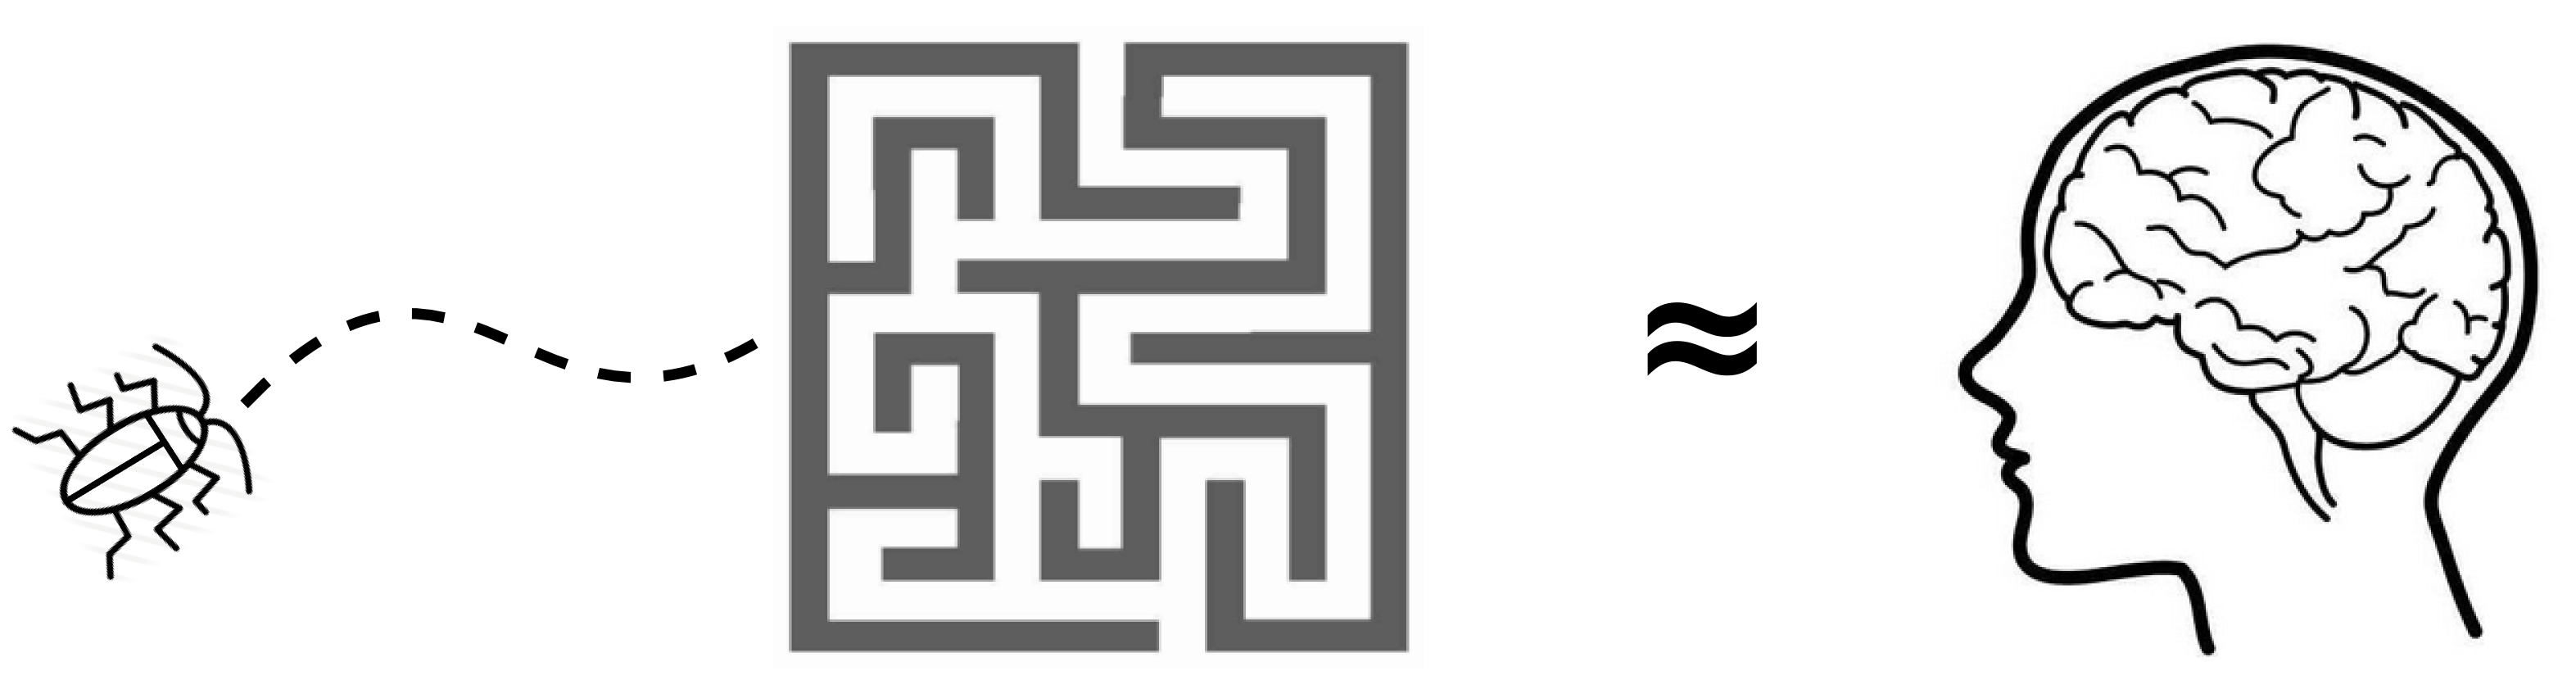
\includegraphics[scale=0.5]{maze-metaphor.png}}}
\end{equation}

The main idea is to regard ``thinking'' as a \emp{dynamical system} operating on \emp{mental states}:
\begin{equation}
\label{fig:mental-state}
\vcenter{\hbox{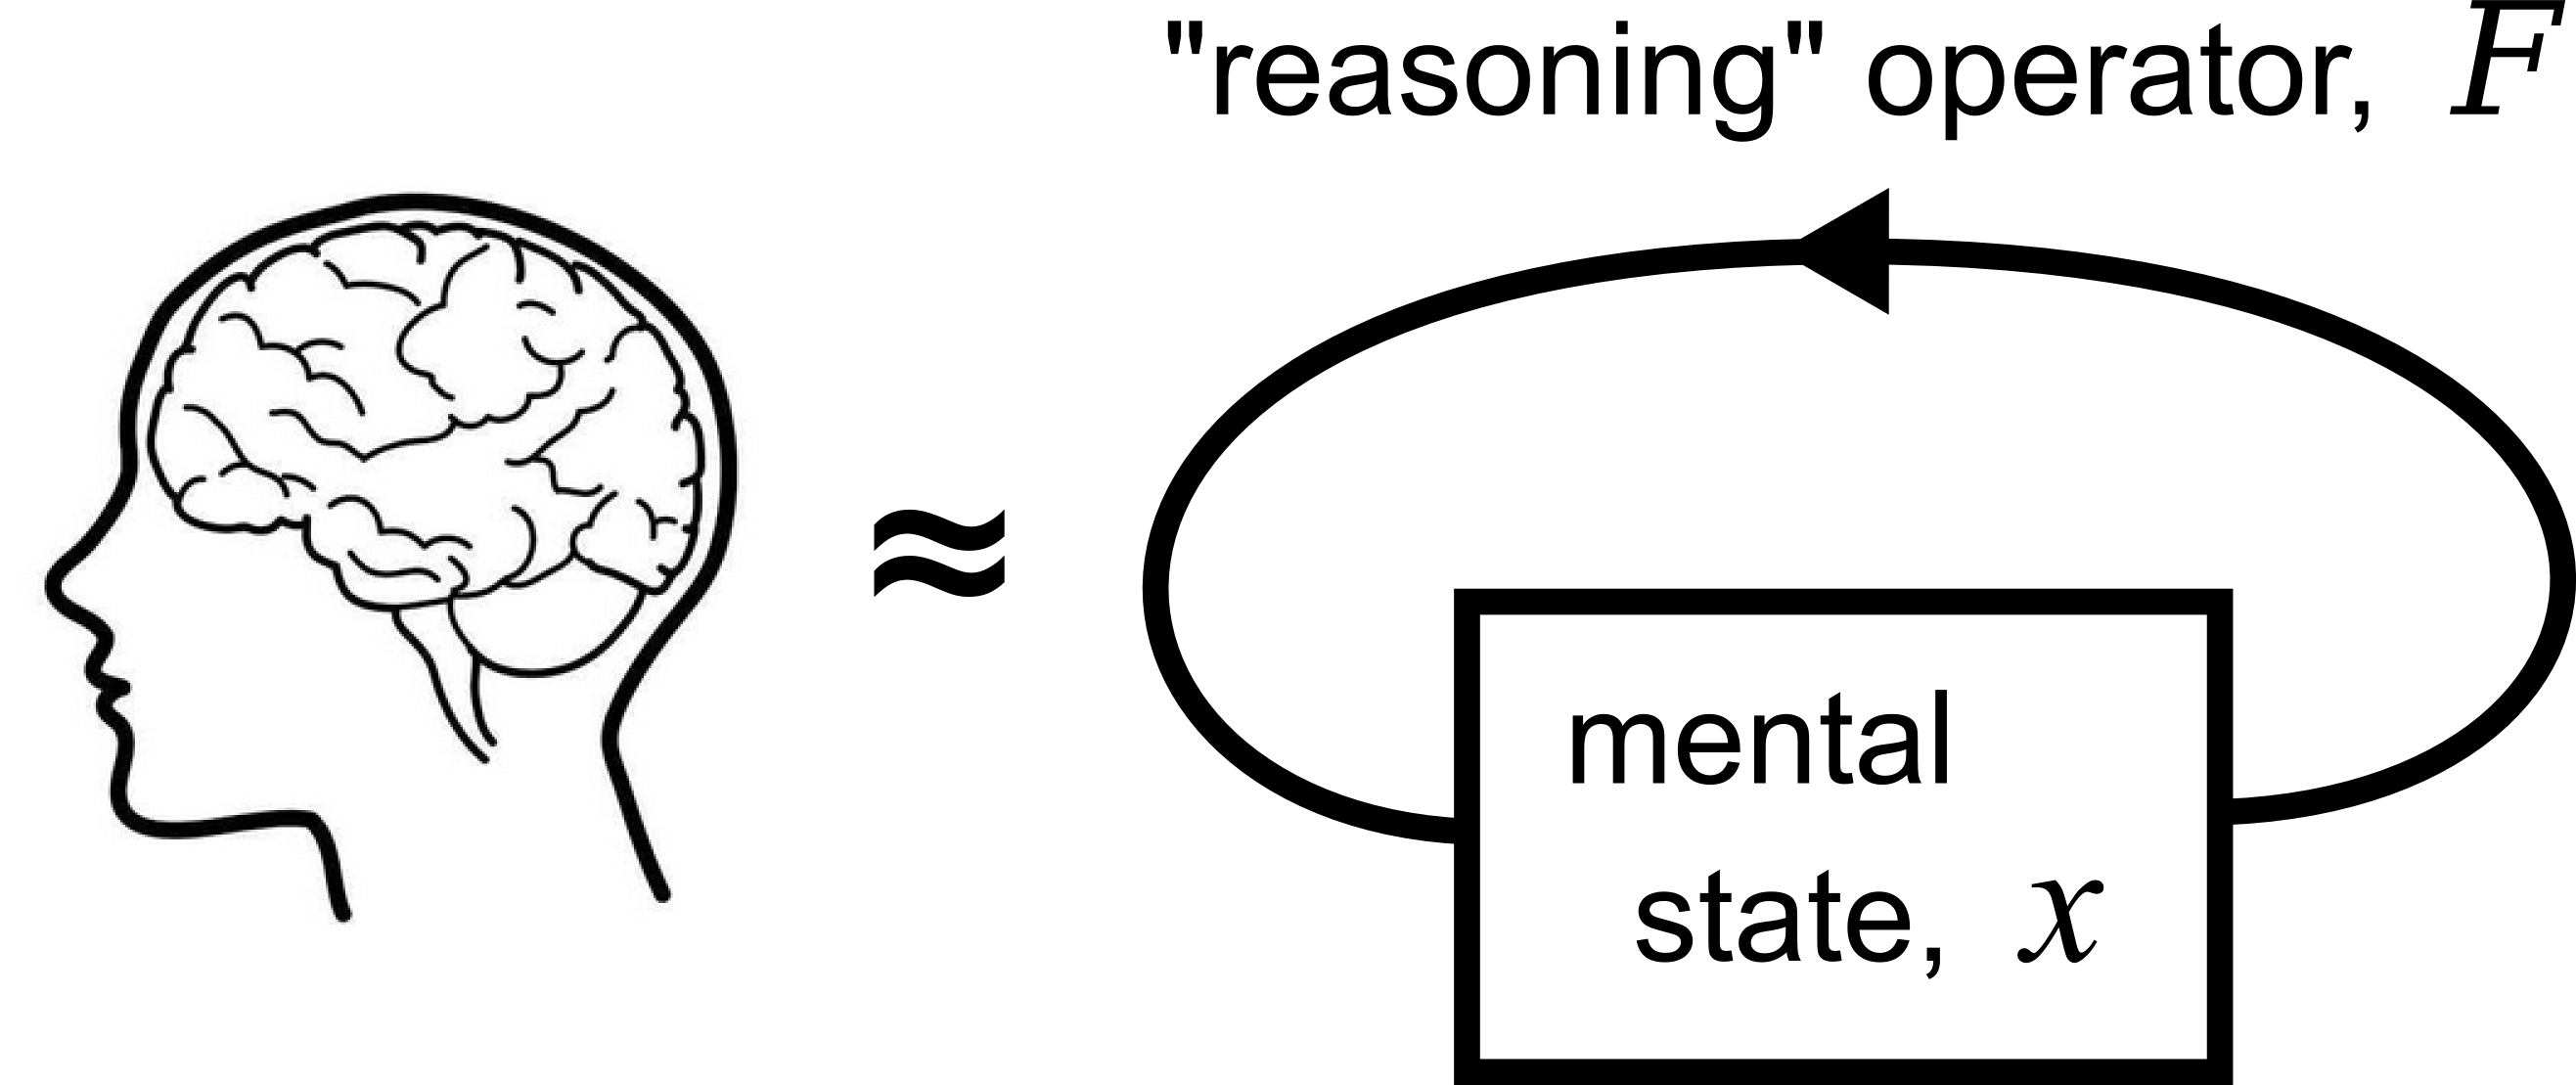
\includegraphics[scale=0.5]{mental-state.png}}}
\end{equation}

A mental state is a \textbf{set of propositions}, for example:
% \renewcommand{\labelitemi}{$\star$}
\begin{itemize}
\item I am in my room, writing a paper for AGI-2019.
\item I am in the midst of writing the sentence, ``I am in my room, ...''
\item I am about to write a gerund phrase ``writing a paper...''
\end{itemize}

Thinking is the process of \emp{transitioning} from one mental state to another.  As I am writing now, I use my mental states to keep track of where I am at within the sentence's syntax, so that I can construct my sentence grammatically.

%The following 3 disciplines are actually synonymous:
%\begin{itemize}
%\item in artificial intelligence, \textbf{reinforcement learning (RL)}
%\item in operations research, \textbf{dynamic programming}
%\item in modern control theory, the \textbf{state space} description
%\end{itemize}

%\begin{itemize}
%\item numerical optimization (eg gradient descent)
%\item differential equations governing time evolution
%\item dynamical systems theory, control theory, dynamic programming, reinforcement learning
% \item Lie algebra and $C^*$-algebra of continuous operators
% \item matrix theory, iteration and fixed-point theory
%\item neural networks and deep learning ... etc.
%\end{itemize}

%=======================================================================================
\begin{comment}

\subsection{Related work}

Google's \textbf{PageRank} is one of the earlier successful applications of vector-space and matrix techniques.  The \textbf{Word2Vec} \cite{Weston2015} algorithm that maps natural-language words to vectors is also spectacularly successful and influential;  it demonstrated the potential advantages of vector representations.  As for reinforcement learning, Q-learning (a form of RL) has been combined with deep learning to successfully play Atari games \cite{Mnih2013};  Their architecture is exactly the same as ours, except that we are trying to refine the internal structure of the learner.
%, both exploit the efficiency of vector and matrix calculus.

This is the cartoon version of our architecture:
\begin{equation}
\vcenter{\hbox{\includegraphics[scale=0.5]{architecture-cartoon.png}}}
\end{equation}

%=======================================================================================
\end{comment}

\subsection{``Introspective'' view of reinforcement learning}

Traditionally, RL deals with acting in an \textit{external} environment; value / utility is assigned to \textit{external} states.  In this view, the \textit{internal} mental state of the agent may change without any noticeable change externally:
\begin{equation}
\vcenter{\hbox{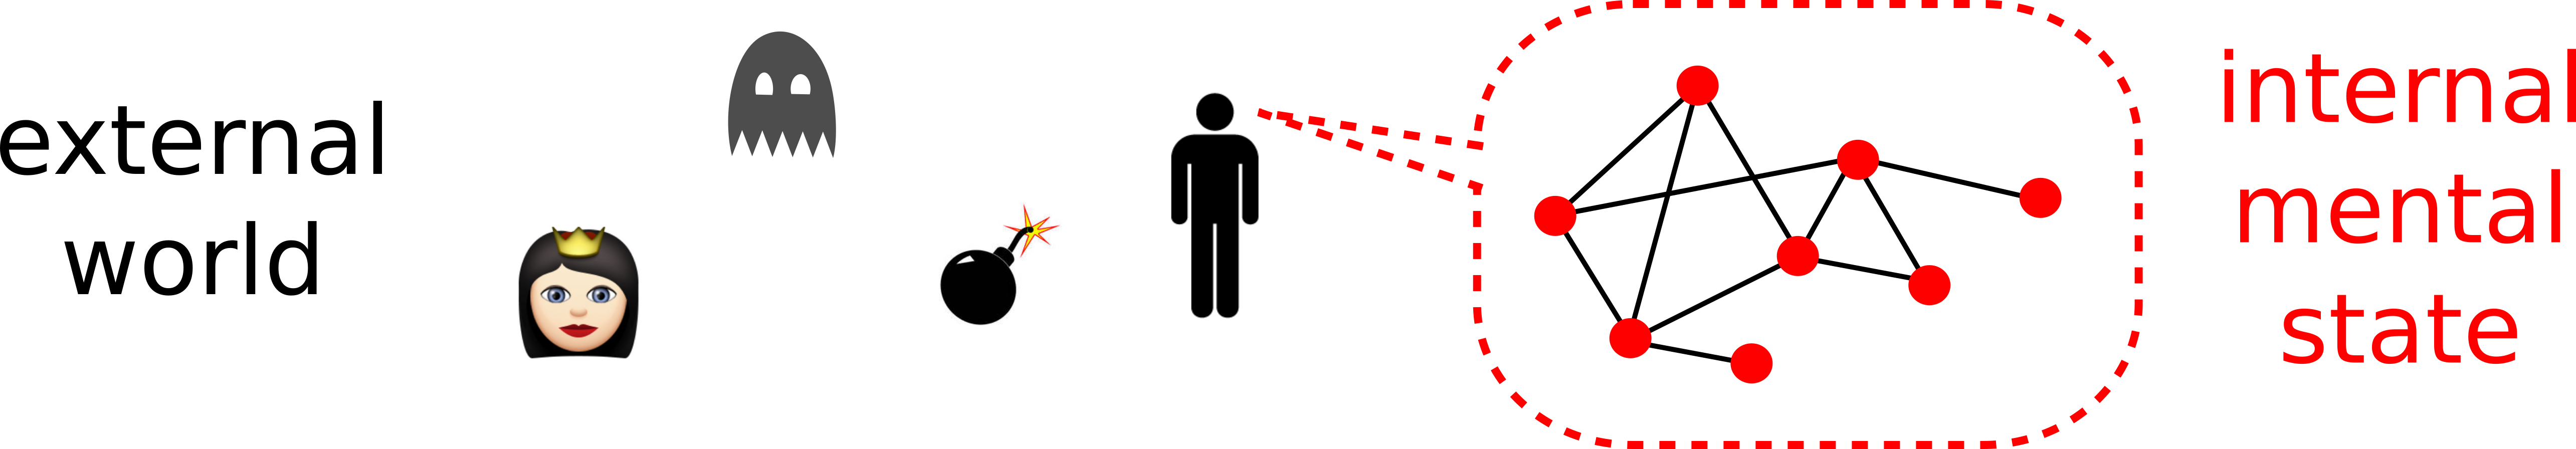
\includegraphics[scale=0.6]{save-princess.png}}}
\end{equation}
% The usefulness of RL (ie, the Bellman update technique) makes me wonder if it'd be advantageous to invert the perspective to consider the internal mental landscape instead.  Then, an internal state would have higher utility when it has been visited by many successful ``thinking'' trajectories.

\subsection{Actions = cognitive state-transitions = ``thinking''}

Our system consists of two main algorithms:
\begin{enumerate}
	\item Learning the transition function $\vdash$ or $\vect{F}: \vect{x} \mapsto \vect{x}'$.  $\vect{F}$ represents the \textbf{knowledge} that constrains thinking.  In other words, the learning of $\vect{F}$ is the learning of ``static'' knowledge.
	\item Finding the optimal trajectory of the state $\vect{x}$.  This corresponds to optimal ``thinking'' under the constraints of static knowledge.
\end{enumerate}

In our architecture, $\vect{F}$ can implemented as a simple feed-forward neural network (where ``deep'' simply means ``many layers''):
\begin{equation}
\vcenter{\hbox{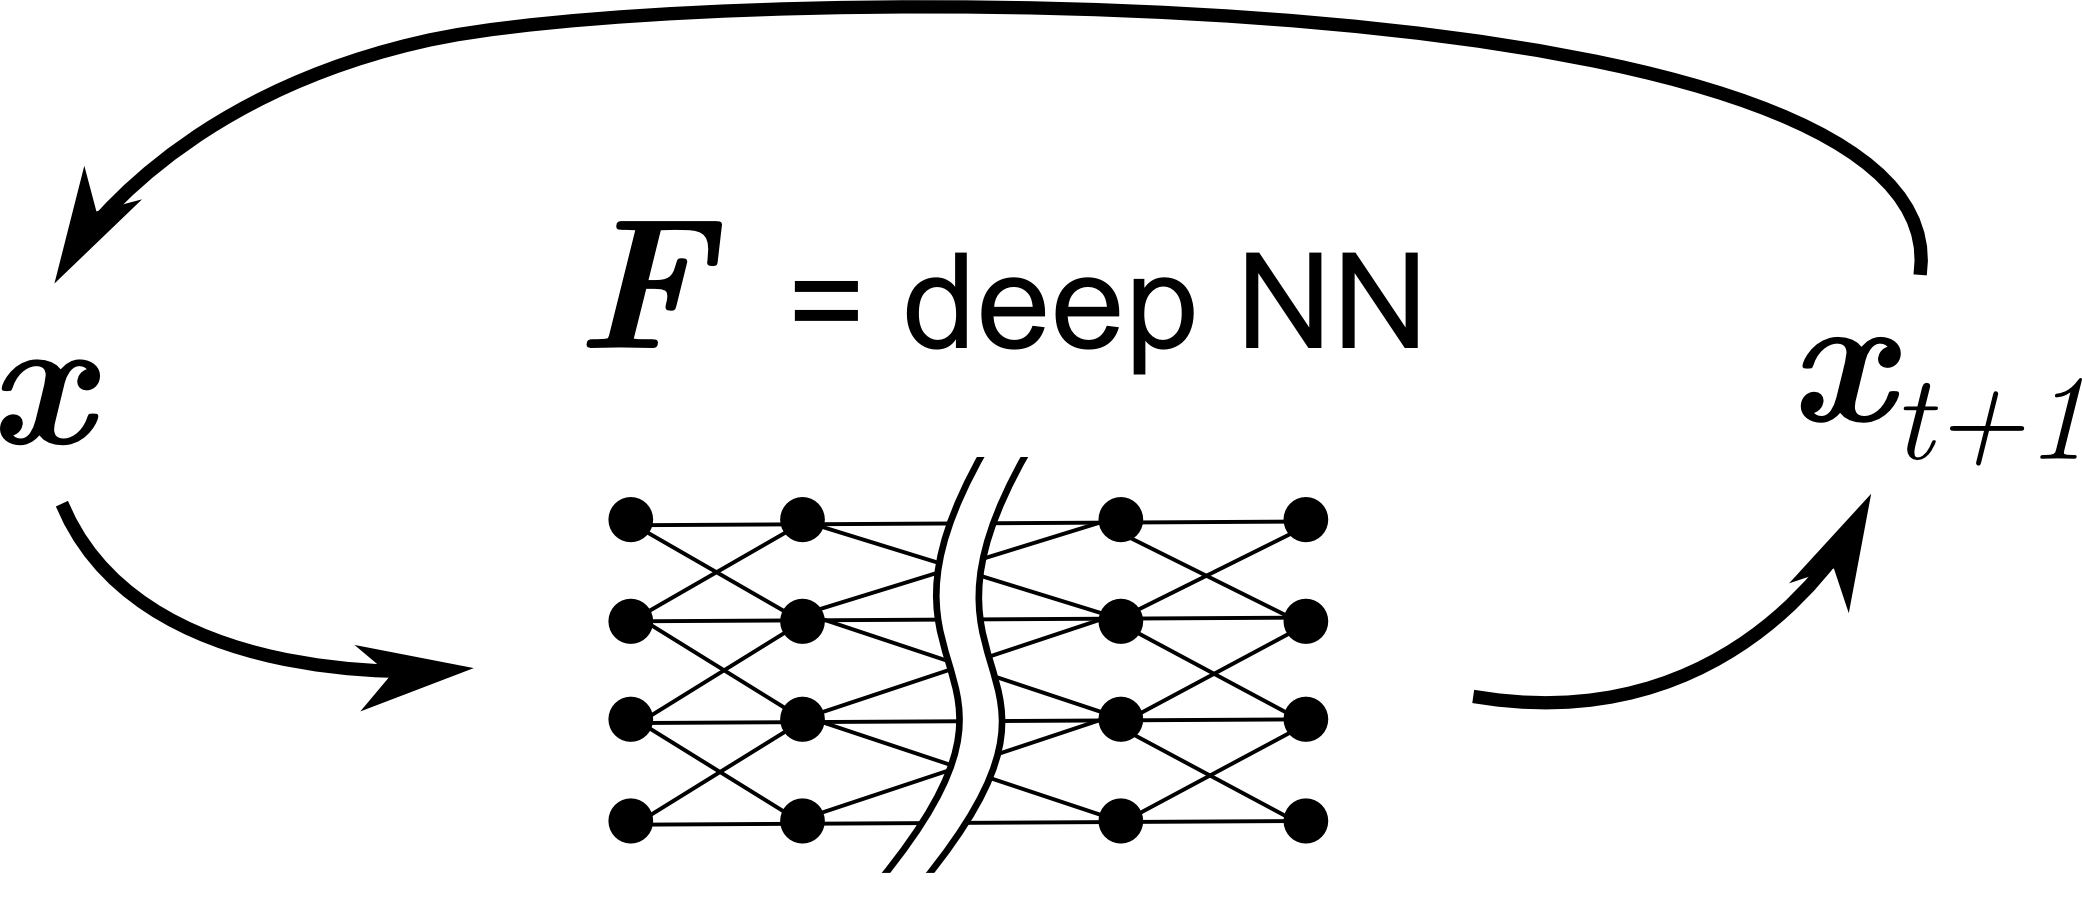
\includegraphics[scale=0.7]{genifer-model-00.png}}}
\end{equation}

In this minimal architecture there is no \textbf{episodic memory}, but this does not seem to be a bottleneck problem. %\textit{The structure of memory} \cite{YanMemory}.

\subsection{Comparison with AIXI}

AIXI's environmental setting is the same as ours, but its agent's internal model is a universal Turing machine, and the optimal action is chosen by maximizing potential rewards over all programs of the UTM.  In our (minimal) model, the UTM is \uline{constrained} to be a neural network, where the NN's \textbf{state} is analogous to the UTM's \textbf{tape}, and the optimal weights (program) are found via Bellman optimality.

\subsection{Control-theoretic setting}

The cognitive state is a vector $\vect{x} \in \mathbb{X}$ where $\mathbb{X}$ is the space of all possible cognitive states, the reasoning operator $\vdash$ or $\vect{F}$ is an \textbf{endomorphism} (an \textbf{iterative map}) $\mathbb{X} \rightarrow \mathbb{X}$.

Mathematically this is a \emp{dynamical system} that can be defined by:
\begin{eqnarray}
\boxed{\mbox{discrete time}} \quad \quad & \vect{x}_{t+1} = \vect{F}(\vect{x}_t) \label{eqn0}\\
\mbox{or } \boxed{\mbox{continuous time}} \quad \quad & \dot{\vect{x}} = \vect{f}(\vect{x}) \label{eqn1}
\end{eqnarray}
%($\vect{F}$ is implemented as the deep learning network in our approach.)
where $\vect{f}$ and $\vect{F}$ are different but related
\footnote{They are related by: $\vect{x}(t + 1) = \vect{F}(\vect{x}(t))$, $\vect{x}^{-1}(\vect{x}(t)) = t =  \int^{\vect{x}_t}_{\vect{x}_0} \frac{d\vect{x}}{\vect{f}(\vect{x}(t))}$, and $f(\vect{x}) = \frac{1}{(\vect{x}^{-1})'(\vect{x}(t))}$.  So we can just solve the functional equation $\vect{x}^{-1}(\vect{F}(\vect{x})) - \vect{x}^{-1}(\vect{x}) = 1$. See \cite{Dolotin2007} \S8.2.3.
}.
For ease of discussion, sometimes I mix discrete-time and continuous-time notations.

A \emp{control system} is a dynamical system added with the control vector $\vect{u}(t)$:
\begin{equation}
\label{eqn:control-rule}
\dot{\vect{x}}(t) = \vect{f}(\vect{x}(t), {\color{red} \vect{u}(t)}, t) .
\end{equation}
The goal of control theory is to find the optimal $\vect{u}^*(t)$ function, such that the system moves from the initial state $\vect{x}_0$ to the terminal state $\vect{x_\bot}$.

\begin{comment}
A typical control-theory problem is described by:
\begin{eqnarray}
\boxed{\mbox{state equation}} \quad & \dot{\vect{x}}(t) = \vect{f}[\vect{x}(t), \vect{u}(t), t] \label{eqn1}\\
\boxed{\mbox{boundary condition}} \quad & \vect{x}(t_0) = \vect{x}_0 \,,\, \vect{x}(t_\bot) = \vect{x}_\bot \\
\boxed{\mbox{objective function}} \quad & J = \int_{t_0}^{t_\bot} L[\vect{x}(t), \vect{u}(t), t] dt
\end{eqnarray}
and we seek the optimal control $\vect{u}^*(t)$.
\end{comment}

%According to control theory, the condition for \textbf{optimal path} is given by the Hamilton-Jacobi-Bellman equation:
%\begin{equation}
%\boxed{\mbox{Hamilton-Jacobi-Bellman}} \quad
%0 = \frac{\partial J^*}{\partial t} + \min_u H
%\end{equation}
%\frac{d}{dt} V(x,t) = \min_u \{ C(x,u) + \langle \nabla V(x,t), f(x,u) \rangle \} 

% In the next section %\S\ref{sec:quantum}
% we shall look into the meaning of $J$, $L$, and $H$.

\begin{comment}
\subsection{Reinforcement learning / dynamic programming}

\textbf{Reinforcement learning} is a branch of machine learning that is particularly suitable for controlling an \textbf{autonomous agent} who interacts with an \textbf{environment}.  It uses \textbf{sensory perception} and \textbf{rewards} to continually modify its \textbf{behavior}.  The exemplary image you should invoke in mind is that of a small insect that navigates a maze looking for food and avoiding predators:  $\vcenter{\hbox{
\includegraphics[scale=0.1]{cockroach.png}}}$

A reinforcement learning system consists of a 4-tuple:
\begin{equation}
\boxed{\mbox{reinforcement learning system}} \; = (\vect{x} \in \mbox{States}, \vect{u} \in \mbox{Actions}, R = \mbox{Rewards}, \pi = \mbox{Policy})
\end{equation}
For details readers may see my \textit{Reinforcement learning tutorial} \cite{YanRLtutorialEN}.

%is synonymous with \textbf{dynamic programming}, which is also the main content of modern \textbf{control theory} with the state-space description.

$U$ is the total rewards of a sequence of actions:
%\begin{equation}
%\boxed{\mbox{total value of state 0}} \; U(\vect{x}_0) = \sum_t \; \boxed{\mbox{reward at time t}} \; R(\vect{x}_t, \vect{u}_t)
%\end{equation}
\begin{eqnarray}
\mbox{\footnotesize total value of state 0} \tikzmark{uu} & \quad \quad \quad & \mbox{\footnotesize reward at time $t$} \tikzmark{rr} \nonumber \\
\nonumber \\
\tikzmark{UU} U(\vect{x}_0) & = & \sum_t \; \tikzmark{RR} R(\vect{x}_t, \vect{u}_t)
\begin{tikzpicture}[overlay,remember picture]
  \draw (uu.center) +(-50pt,-3pt) -- ([shift={(4pt,12pt)}]UU.center);
  \draw (rr.center) +(-35pt,-3pt) -- ([shift={(8pt,12pt)}]RR.center);
\end{tikzpicture}
\end{eqnarray}
For example, the value of playing a chess move is not just the immediate reward of that move, but includes the consequences of playing that move (eg, greedily taking a pawn now may lead to checkmate 10 moves later).  Or, faced with delicious food, some people may choose not to eat, for fear of getting fat.

%The goal of \textbf{reinforcement learning} is to learn the \emp{policy function}:
%\begin{equation}
%\begin{tikzcd}[]
%\mbox{policy : ~~state} \arrow[r, mapsto, "\scalebox{0.8}{action}"] & \mbox{state'}
%\end{tikzcd}
%\end{equation}
%when we are given the \emp{state space}, \emp{action space}, and \emp{reward function}:
%\begin{equation}
%\mbox{reward}: \boxed{\mbox{state}} \times \boxed{\mbox{action}} \rightarrow \mathbb{R}
%\end{equation}
%The action $a$ is the same notion as the control variable $u$ in control theory.

The central idea of \textbf{Dynamic programming} is the \textbf{Bellman optimality condition}, % Richard Bellman in 1953 proposed this formula, while he was working at RAND corporation, dealing with operations research problems.
% The \textbf{Bellman condition} 
which says:  ``\uline{if we cut off a tiny bit from the endpoint of the optimal path, the remaining path is still an optimal path between the new endpoints}.''

\begin{eqnarray}
& \mbox{\footnotesize value of entire path} \tikzmark{uEntire} \quad \quad \mbox{\footnotesize reward of choosing $\vect{u}$ at current state} \tikzmark{rCurrent} \quad \quad \mbox{\footnotesize value of rest of path} \tikzmark{uRest} \nonumber \\
\nonumber \\
& \boxed{\mbox{Bellman equation}} \quad \tikzmark{UEntire} U^*(\vect{x}) = \max\limits_{\vect{u}} \{ \; \tikzmark{RCurrent} R(\vect{u}) + \tikzmark{URest} U^*(\vect{x}_{t+1}) \; \}
\begin{tikzpicture}[overlay,remember picture]
  \draw (uEntire.center) +(-30pt,-3pt) -- ([shift={(4pt,12pt)}]UEntire.center);
  \draw (rCurrent.center) +(-80pt,-3pt) -- ([shift={(4pt,12pt)}]RCurrent.center);
  \draw (uRest.center) +(-65pt,-3pt) -- ([shift={(8pt,12pt)}]URest.center);
\end{tikzpicture}
\end{eqnarray}
This seemingly simple formula is the \uline{entire content} of dynamic programming;  What it means is that:  When seeking the path with the best value, we cut off a bit from the path, thus reducing the problem to a smaller problem;  In other words, it is a \textbf{recursive relation} over time.

In AI reinforcement learning there is an oft-employed trick known as $Q$-learning.  $Q$ value is just a variation of $U$ value;  there is a $U$ value for each state, and $Q$ is the \textbf{decomposition} of $U$ by all the actions available to that state.  In other words, $Q$ is the utility of doing action $\vect{u}$ in state $\vect{x}$.  The relation between $Q$ and $U$ is:
\begin{equation}
U(\vect{x}) = \max\limits_{\vect{u}} \, Q(\vect{x}, \vect{u})
\end{equation}
The advantage of $Q$ is the ease of learning.  We just need to learn the value of actions under each state.  This is so-called ``\textbf{model free learning}''.

%The \emp{Bellman equation} governs reinforcement learning just as in control theory:
%\begin{eqnarray}
%\boxed{\mbox{optimal path}} = & \mbox{choose max reward on current path segment} \nonumber \\
%& \quad + \boxed{\mbox{the rest of optimal path}}
%\end{eqnarray}
%In math notation:
%\begin{equation}
%U^*_t = \max_{u} \{ \; \boxed{\mbox{reward}(u, t)} + U^*_{t-1} \; \}
%\end{equation}
%where $U$ is the ``long-term value'' or \emp{utility} of a path.

%Conceptually, $U$ is the \textbf{integration} of instantaneous rewards over time:
%\begin{equation}
%\boxed{\mbox{utility, or value} U} = \int \boxed{\mbox{reward} R} \,dt
%\end{equation}
\end{comment}

\begin{comment}
%==================================================================================
Under the reinforcement learning framework, intelligence is decomposed into \textbf{thinking} and \textbf{learning}:
\begin{itemize}
\item \emp{Thinking} means finding the optimal trajectory of $\vect{x}$ according to the \textbf{knowledge} stored in the deep NN.  This is achieved using the Bellman equation to calculate $\vect{u}^*$.  The trajectory of $\vect{x}$ is constrained by the deep NN (in other words, the system must think in accordance with \textbf{correct knowledge}).  While thinking, the deep NN stays \textbf{constant}.

\item \emp{Learning} means learning the weights in the deep NN.  Changing $W$ changes $\vect{F}$, which determines the state equation (\ref{eqn0}), so the entire system becomes a new one.  In other words, deep NN learning is a kind of \textbf{second-order learning}:  Consider 2 systems $\vect{F}$ and $\vect{F} + \epsilon \hat{\vect{F}}$, after \uline{many trials} of thinking with different premises, if the average reward is higher in the altered system, $\vect{F}$ will learn towards the $\hat{\vect{F}}$ direction.
% 即是根据已学得的\textbf{知识}(知识储存在 deep NN 里),在思维空间中找寻 $\vect{x}$ 最优的轨迹,方法是根据 Bellman 方程计算 $\vect{u}^*$。 $\vect{x}$ 的轨迹受 deep NN 约束(亦即是说,系统只能依据\textbf{正确的知识}去思考),思考时 deep NN 是\textbf{不变}的。
%\item \emp{学习}就是学习神经网络 deep NN 的 weights $W_\ell$,改变 $W$ 即改变 $\vect{F}$,而$\vect{F}$ 决定\textbf{状态方程} (\ref{eqn0}),所以整个系统变了另一个系统。 换句话说,deep NN 的学习是一种 \textbf{second-order learning}: 考虑两个系统 $\vect{F}$ 和 $\vect{F} + \epsilon \hat{\vect{F}}$,经过很多次思考过程,如果奖励的平均值在后者有所增加,则 $\vect{F}$ 向 $\hat{\vect{F}}$ 方向学习。
\end{itemize}
%==================================================================================
\end{comment}

\subsection{Lagrangians and Hamiltonians}
\label{sec:Langrangians-Hamiltonians}
%\subsection{Control theory / dynamical systems theory}

%This section is optional.

In \emp{reinforcement learning}, we are concerned with two quantities:
\begin{itemize}
	\item $r(\vect{x}, \vect{u})$ = \emp{reward} of doing action $\vect{u}$ in state $\vect{x}$
	\item $U(\vect{x})$ = \emp{utility} or \emp{value} of state $\vect{x}$ 
\end{itemize}
where \textbf{utility} is the integral of instantaneous \textbf{rewards} over time:
\begin{equation}
\boxed{\mbox{utility} $U$} = \int \boxed{\mbox{reward} $r$} \,dt .
\end{equation}
%(价值有时用 $V$ 表示,但为避免和势能 $V$ 混淆故不用。)

%In \emp{control-theoretic} parlance, it is usually defined the \textbf{cost functional}:
%\begin{equation}
%\boxed{\mbox{cost } $J$} = \int L dt + \Phi(\vect{x}_\bot)
%\end{equation}
%where $L$ is the \textbf{running cost}, ie, the cost of making each step; 
%$\Phi$ is the \textbf{terminal cost}, ie, the value when the terminal state $\vect{x}_\bot$ is reached.

%Define a continuous version of ``utility'':
%\begin{equation}
%V(x,t) = \min_u \{ \int_t^{t_\bot} C(x,u)dt + \Phi(x_\bot,t_\bot) \} 
%\end{equation}
%where $t$ is time, $u$ is a set of control parameters, $C$ is the \emp{cost-rate} function:
%\begin{equation}
%\int C dt = R = \mbox{reward}
%\end{equation}
%This integral expresses the ``cost of the path'', whereas $\Phi(x_\bot,t_\bot)$ is the ``cost at termination''.

%In \emp{analytical mechanics} $L$ is known as the \textbf{Lagrangian}, and the time-integral of $L$ is called the \textbf{action}:
%\begin{equation}
%\boxed{\mbox{action } $S$} = \int L dt
%\end{equation}
%Hamilton's \emp{principle of least action} says that $S$ always takes the \textbf{stationary value}, ie, the $S$ value is extremal compared with neighboring trajectories.

%The \textbf{Hamiltonian} is defined as $\displaystyle H = L + \frac{\partial J^*}{\partial \vect{x}} \vect{f}$, which arises from the method of \textbf{Lagrange multipliers}.  % For details please refer to my \textit{Control theory tutorial}\cite{YanControlTheoryTutorial}.

%All these refer to essentially the same thing, so we have the following correspondence:

There is a well-known correspondence between control theory, dynamic programming (reinforcement learning), and analytical mechanics, observed by Kalman and Pontryagin, among others (\textit{cf} the textbook \cite{Liberzon2012}):
\setlength{\tabcolsep}{0.5em} % for the horizontal padding
{\renewcommand{\arraystretch}{1.2}
\begin{equation}
\begin{tabular}{|c|c|c|}
\hline 
\emp{Reinforcement learning} & \emp{Control theory} & \emp{Analytical mechanics} \\ 
\hline
value $V$ or utility $U$ & cost $J$ & action $S$ \\ 
\hline 
instantaneous reward $r$ & running cost $L$ & Lagrangian $L$ \\ 
\hline 
action $\vect{a}$ & control $\vect{u}$ & (external force) \\
\hline
 & Lagrange multiplier $\vect{\lambda}$ & momentum $\vect{p}$ \\
\hline
$ U = \int R \,dt$ & $ J = \int L \,dt + \Phi(\vect{x}_\bot)$ & $ S = \int L \,dt$ \\
\hline
\end{tabular} 
\end{equation}
}
$\Phi$ is the \textbf{terminal cost}, ie, the value when the terminal state $\vect{x}_\bot$ is reached.

Interestingly, the reward $r$ corresponds to the \textbf{Lagrangian} in physics, whose unit is ``energy'';  In other words, ``desires'' or ``happiness'' appear to be measured by units of ``energy'', this coincides with the idea of ``positive energy'' in pop psychology.  Whereas, long-term value is measured in units of $[\mbox{energy} \times \mbox{time}]$.

The \textbf{Hamiltonian} can be defined by
\begin{equation}
\label{eqn:def-Hamiltonian}
H := \langle \vect{p}, \vect{f} \rangle - L
\end{equation}
which arises from the \textbf{Lagrange multiplier} $\vect{\lambda} \equiv \vect{p}$.  It can be shown that, at the optimum,
\begin{equation}
\vect{\lambda} = \frac{\partial J^*}{\partial \vect{x}}
    \quad \mbox{ or } \quad 
\vect{p} = \frac{\partial S}{\partial \vect{x}}
\end{equation}
where ${}^*$ refers to the extremum, and $\langle \cdot, \cdot \rangle$ is the inner product.

%用比较浅显的例子: 和美女做爱能带来即时的快感 (= 奖励 $R$),但如果强奸的话会坐牢,之后很长时间很苦闷,所以这个做法的长远价值 $U$ 比其他做法较低,正常人不会选择它。

In the classical \textbf{variational calculus}, the \textbf{optimal path} is given by the condition:
\begin{equation}
\label{eqn:variational-calculus}
\boxed{\mbox{variational calculus}} \quad
\frac{\partial H}{\partial \vect{u}} = 0
\end{equation}
which is later generalized by Pontryagin as the \textbf{maximum principle}:
\begin{equation}
\label{eqn:maximum-principle}
\boxed{\mbox{Pontryagin}} \quad
H^* = \inf_{u \in \mathbb{U}} H(\vect{x}^*, \vect{\lambda}^*, \vect{u}, t)
\end{equation}
and also roughly equivalently to the \textbf{Hamilton-Jacobi-Bellman equation}:
%The equation of motion for the continuous-time case is the famed \emp{Hamilton-Jacobi-Bellman equation}:
% \footnote{To digress a bit, this equation is also analogous to the \emp{Schr\"{o}dinger equation} in quantum mechanics:
%\begin{equation}
%i \hbar \frac{\partial}{\partial t} \Psi(x,t) = \left[ V(x,t) + \frac{-\hbar^2}{2\mu} \nabla^2 \right] \Psi(x,t).
%\end{equation}
%where $\Psi$ is analogous to our $U$ (perhaps $\Psi$ is something that nature wants to optimize?)}
\begin{equation}
\label{eqn:HJB}
\boxed{\mbox{Hamilton-Jacobi-Bellman}} \quad
\frac{\partial S^*}{\partial t} = -\inf_u H = -\inf_u \left\{ L + \bigg\langle \frac{\partial S^*}{\partial \vect{x}}, \vect{u} \bigg\rangle \right\} .
\end{equation}

Traditional logic-based AI systems are discrete-time; changing them to continuous-time seems to merely increase the computational burden and is \textit{ungainful}.  But the time-critical step is the learning of $\vect{u}$, which may be solved via (\ref{eqn:variational-calculus}), (\ref{eqn:maximum-principle}), or (\ref{eqn:HJB}).  
% The recent advent of \textbf{symplectic integrators} \cite{Leimkuhler2009} are known to produce better numerical solutions that retain qualitative features of the exact solution, eg. quasi-periodicity.

From the author's limited knowledge in control theory, it seems we currently don't have efficient algorithms to sovle the HJB equation, but the maximum principle (\ref{eqn:maximum-principle}) is more useful in practice, though it requires the Hamiltonian to be defined in addition to the Lagrangian.  Current deep-learning RL literature seems to focus on using the reward (\textit{ie}, Lagrangian), so they have objective functions like the form in (\ref{eqn:policy-gradient}), which is cumbersome as the total value $V$ is itself a summation inside another summation over all trajectories.  Gradient descent $\nabla_{\vect{u}}$ against the Hamiltonian $H$ may be computationally more efficient.

%一个智能系统,它有「智慧」的条件,就是每时每刻都不断追求「开心能量」或奖励 $R$ 的最大值,但它必需权衡轻重,有计划地找到长远的效用 $U$ 的最大值。

% This correspondence between these 3 theories is explained in detail in Daniel Liberzon's book \cite{Liberzon2012}.  

\begin{comment}
%==================================================================================
An interesting insight from control theory is that our system is a Hamiltonian dynamical system in a broad sense.

Hamilton's \emp{principle of least action} says that the trajectories of dynamical systems occuring in nature always choose to have their action $S$ taking \textbf{stationary values} when compared to neighboring paths.  The action is the time integral of the Lagrangian $L$:
\begin{equation}
\boxed{\mbox{Action} S} = \int \boxed{\mbox{Lagrangian} L} \; dt
\end{equation}
From this we see that the Lagrangian corresponds to the instantaneous ``rewards'' of our system.  It is perhaps not a coincidence that the Lagrangian has units of \textbf{energy}, in accordance with the folk psychology notion of ``positive energy'' when we talk about desirable things.

The \emp{Hamiltonian} $H$ arises when we consider a typical control theory problem;  The system is defined via:
\begin{eqnarray}
\mbox{state equation:} \quad & \dot{\vect{x}}(t) = \vect{f}[\vect{x}(t), \vect{u}(t), t] \\
\mbox{boundary condition:} \quad & \vect{x}(t_0) = \vect{x}_0 \,,\, \vect{x}(t_\bot) = \vect{x}_\bot \\
\mbox{objective function:} \quad & J = \int_{t_0}^{t_\bot} L[\vect{x}(t), \vect{u}(t), t] dt
\end{eqnarray}
The goal is to find the optimal control $\vect{u}^*(t)$.

Now apply the technique of \emp{Lagrange multipliers} for finding the maximum of a function, this leads to the new objective function:
\begin{equation}
U = \int_{t_0}^{t_\bot} \{ L + \vect{\lambda}^T(t) \left[ f(\vect{x}, \vect{u}, t) - \dot{\vect{x}} \right] \} dt
\end{equation}
So we can introduce a new scalar function $H$, ie the Hamiltonian:
\begin{equation}
H(\vect{x}, \vect{u}, t) = L(\vect{x}, \vect{u}, t) + \vect{\lambda}^T(t) f(\vect{x}, \vect{u}, t)
\end{equation}
Physically, the unit of $\vect{f}$ is velocity, while the unit of $L$ is energy, therefore $\vect{\lambda}$ should have the unit of \emp{momentum}.  This is the reason why the phase space is made up of the diad of $(\mbox{position}, \mbox{momentum})$.

%==================================================================================
\end{comment}

\subsection{Constrained vs unconstrained dynamics}

%In traditional reinforcement learning (left view), the system chooses an action $\vect{a}$, and the transition function $\vect{F}$ gives the probability of reaching each state $\vect{x}$ given action $\vect{a}$.  In our model (right view), all possible cognitive states are potentially \textbf{reachable} from any other state, and therefore the action $\vect{a}$ coincides with the next state $\vect{x}'$.
In our formulation, every state is potentially \textbf{reachable} by some logic rule, this corresponds to the picture on the right:
\begin{equation}
\vcenter{\hbox{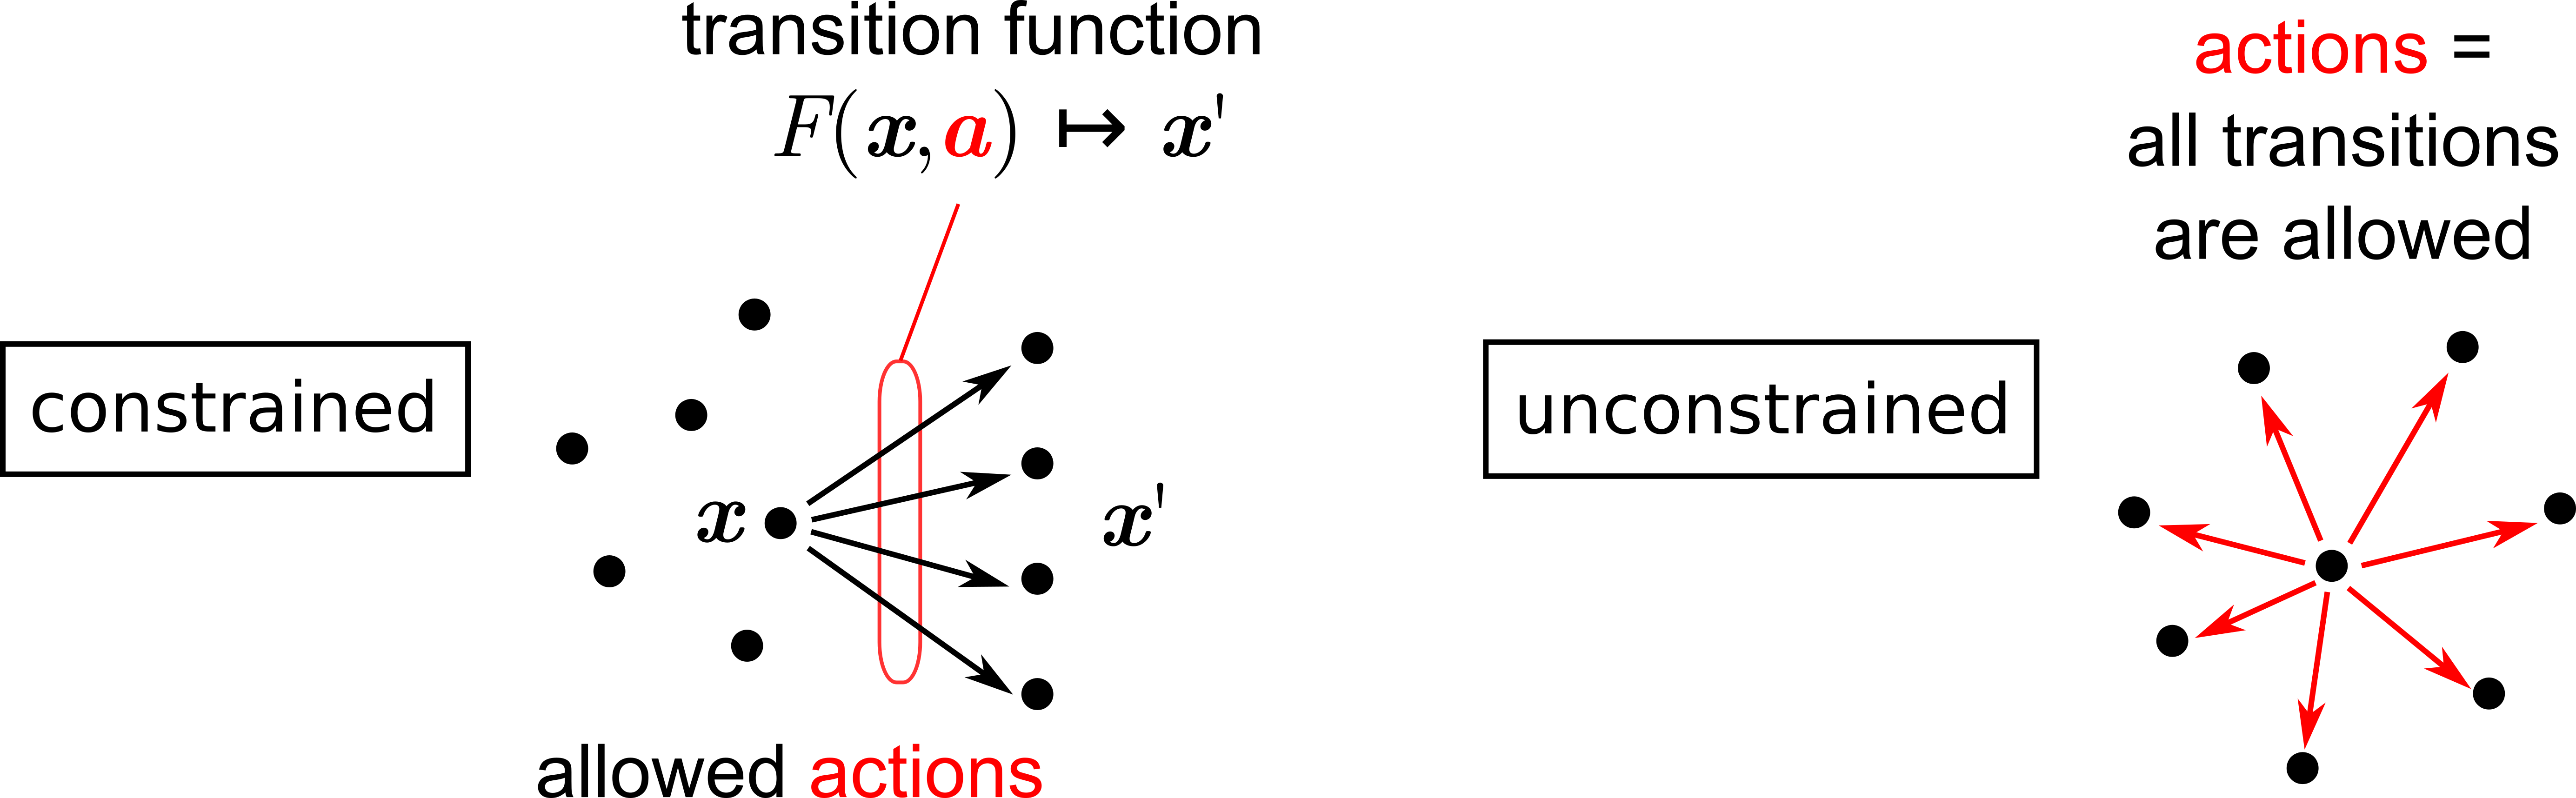
\includegraphics[scale=0.75]{Q-learning-2-views.png}}}
\end{equation}
Under this view, the control rule (\ref{eqn:control-rule}) simplifies to:
\begin{equation}
\dot{\vect{x}} = \vect{f}(\vect{x}, \vect{u}, t) = \vect{u}(t)
\end{equation}
and then the Lagrangian multiplier $\vect{\lambda} \equiv \vect{p}$ follows from (\ref{eqn:def-Hamiltonian}) and (\ref{eqn:variational-calculus}) to be:
\begin{equation}
\vect{\lambda}^* \equiv  \vect{p}^* = \frac{\partial L(t, \vect{x}^*, \vect{u}^*)}{\partial \vect{u}} = \frac{\partial L}{\partial \dot{\vect{x}}}
\end{equation}
which recovers the classical momemtum relation.

%With the substitution $\Psi = e^{i U / \hbar}$ into the HJB equation, one can obtain the
%\emp{Schr\"{o}dinger equation}:
%\begin{equation}
%\boxed{\mbox{Schr\"{o}dinger}} \quad
%i \hbar \frac{\partial \Psi}{\partial t} = \hat{H} \Psi
%\end{equation}
%which means techiques in quantum mechanics can be applied to solve our AGI problem.

\subsection{Policy gradient}

In recent years, the \textbf{policy gradient} method and its variants (\textit{eg} Actor-Critic) has made spectacular success in deep reinforcement learning (DRL).  Basically, the \textbf{stochastic} policy $\pi(\vect{a} | \vect{x})$ is expressed as a function parametrized by $\Theta$ and is updated via:
\begin{equation}
\Theta \stackrel{+}{=} \eta \; \nabla_{\Theta} \widetilde{V}
\end{equation}
where $\eta$ is the \textbf{learning rate}, and $\widetilde{V}$ is the objective function, which is the \textbf{expectation} of the total reward or value $V$ along \textit{all possible} trajectories $\tau$ starting from an initial position:
\begin{equation}
\widetilde{V} = \underset{\tau}{\mathbb{E}}[ \; V(\tau) \;] .
\end{equation}
The gradient of $\widetilde{V}$ can be derived as this formula familiar to practitioners of DRL:
\begin{equation}
\label{eqn:policy-gradient}
\nabla_{\Theta} \widetilde{V} = \nabla_{\Theta} \underset{\tau}{\mathbb{E}}[ \; V(\tau) \;] = \underset{\tau}{\mathbb{E}}[ \; \nabla_{\Theta} \sum_t \log \pi(\vect{a}_t | \vect{x}_t; \Theta) V(\tau) \;] .
\end{equation}

\subsection{Connection with quantum mechanics}
\label{sec:quantum}

Recently, I accidentally discovered
\footnote{The relation $S = i \hbar \log \Psi$ appeared in one of Schr\"{o}dinger's 1926 papers, but is dismissed by him as ``incomprehensible''.  This formula seems to be overlooked by physicists since that time, possibly including Feynman.  I have yet to discuss / verify this with other physicists.}
a precise transition from the classical H-J equation to the \emp{Schr\"{o}dinger equation} in quantum mechanics, via a simple substitution $\Psi = e^{i S / \hbar}$,
\begin{equation}
\begin{tikzcd}[column sep = 6em]
\boxed{\mbox{Hamilton-Jacobi}} \quad \displaystyle \frac{\partial S}{\partial t} = - H \quad
\arrow[Rightarrow, r, "$\Psi = \exp \{ i S / \hbar \} $", align=center]
& \quad \displaystyle i \hbar \frac{\partial \Psi}{\partial t} = H \Psi \quad \boxed{\mbox{Schr\"{o}dinger}} .
\end{tikzcd}
\end{equation} 
This implies that the Schr\"{o}dinger equation is an alternative way of expressing the optimality condition for RL!

%We can also express $J$ using the quantum-mechanical notation:
%\begin{equation}
%J = \langle \Psi | i \hbar \,\log \Psi | \Psi \rangle
%\end{equation}

%All these ``physical'' ideas flow automatically from our definition of \textbf{rewards}, without the need to introduce them artificially.  But these ideas seem not immediately useful to our project, unless we are to explore \textbf{continuous-time} models.

%\subsection{Prior art: other cognitive architectures}

%The minimalist architecture based on reinforcement learning has been proposed by Itimar Ariel from Israel, in 2012 \cite{Arel2012}, and I also independently proposed in 2016 (precursor of this paper).  The prestigious researcher of signal processing, Simon Haykin, recently also used the ``RL + memory'' design, cf. his 2012 book \textit{Cognitive dynamic systems} \cite{Haykin2012}. Vladimir Anashin in the 1990's also proposed this kind of cognitive architecture \cite{Anashin2009}.  There may exist more precedents, eg: \cite{Ivancevic2006}.

\section{Logic structure}

\subsection{Logic is needed as an inductive bias}

The transition function $\vect{F}$ appearing in (\ref{eqn0}) is ``free'' without further restrictions.  The learning of $\vect{F}$ may be slow without further \textbf{induction bias}, \textit{cf} the ``no free lunch'' theorem.  But we know that the transition function is analogous to $\vdash$, the logic consequence or entailment operator.  So we want to impose this logic structure on $\vect{F}$.

By logic structure we mean that $\vect{F}$ would act like a \textbf{knowledge base} $\KB$ containing a large number of logic \textbf{rules}, as in the setting of classical logic-based AI.

\subsection{Geometry induced by logic rules}

A logic rule is a conditional formula with variables.  For example:
\begin{equation}
\forall X \; \forall Y \; \forall Z.  \quad \text{father}({\color{red}X} \tikzmark{p}, {\color{red}Y} \tikzmark{y}) \wedge \mbox{father}({\color{red}Y} \tikzmark{q}, {\color{red}Z} \tikzmark{r}) \Rightarrow \text{grandfather}({\color{red}X} \tikzmark{x}, {\color{red}Z} \tikzmark{z}) 
\begin{tikzpicture}[overlay,remember picture,distance=1.1cm]
\draw[-,red, transform canvas={shift={(-5pt,10pt)}}, out=135,in=45] (x.center) to (p.center);
\draw[-,red, transform canvas={shift={(-5pt,-3pt)}}, out=-20,in=210] (y.center) to (q.center);
\draw[-,red, transform canvas={shift={(-5pt,-3pt)}}, out=-25,in=215] (r.center) to (z.center);
\end{tikzpicture}
\label{linkage-father}
\end{equation}
where the red lines show what I call ``linkages'' between different appearances of the same variables.

\textbf{Quantification} of logic variables, with their linkages, result in \textbf{cylindrical} and \textbf{diagonal} structures when the logic is interpreted \textit{geometrically}.  This is the reason why Tarski discovered the \textbf{cylindric algebra} structure of first-order predicate logic.  Cylindrical shapes can arise from quantification as illustrated below:
\begin{equation}
\label{eqn:cylindric-shapes}
\vcenter{\hbox{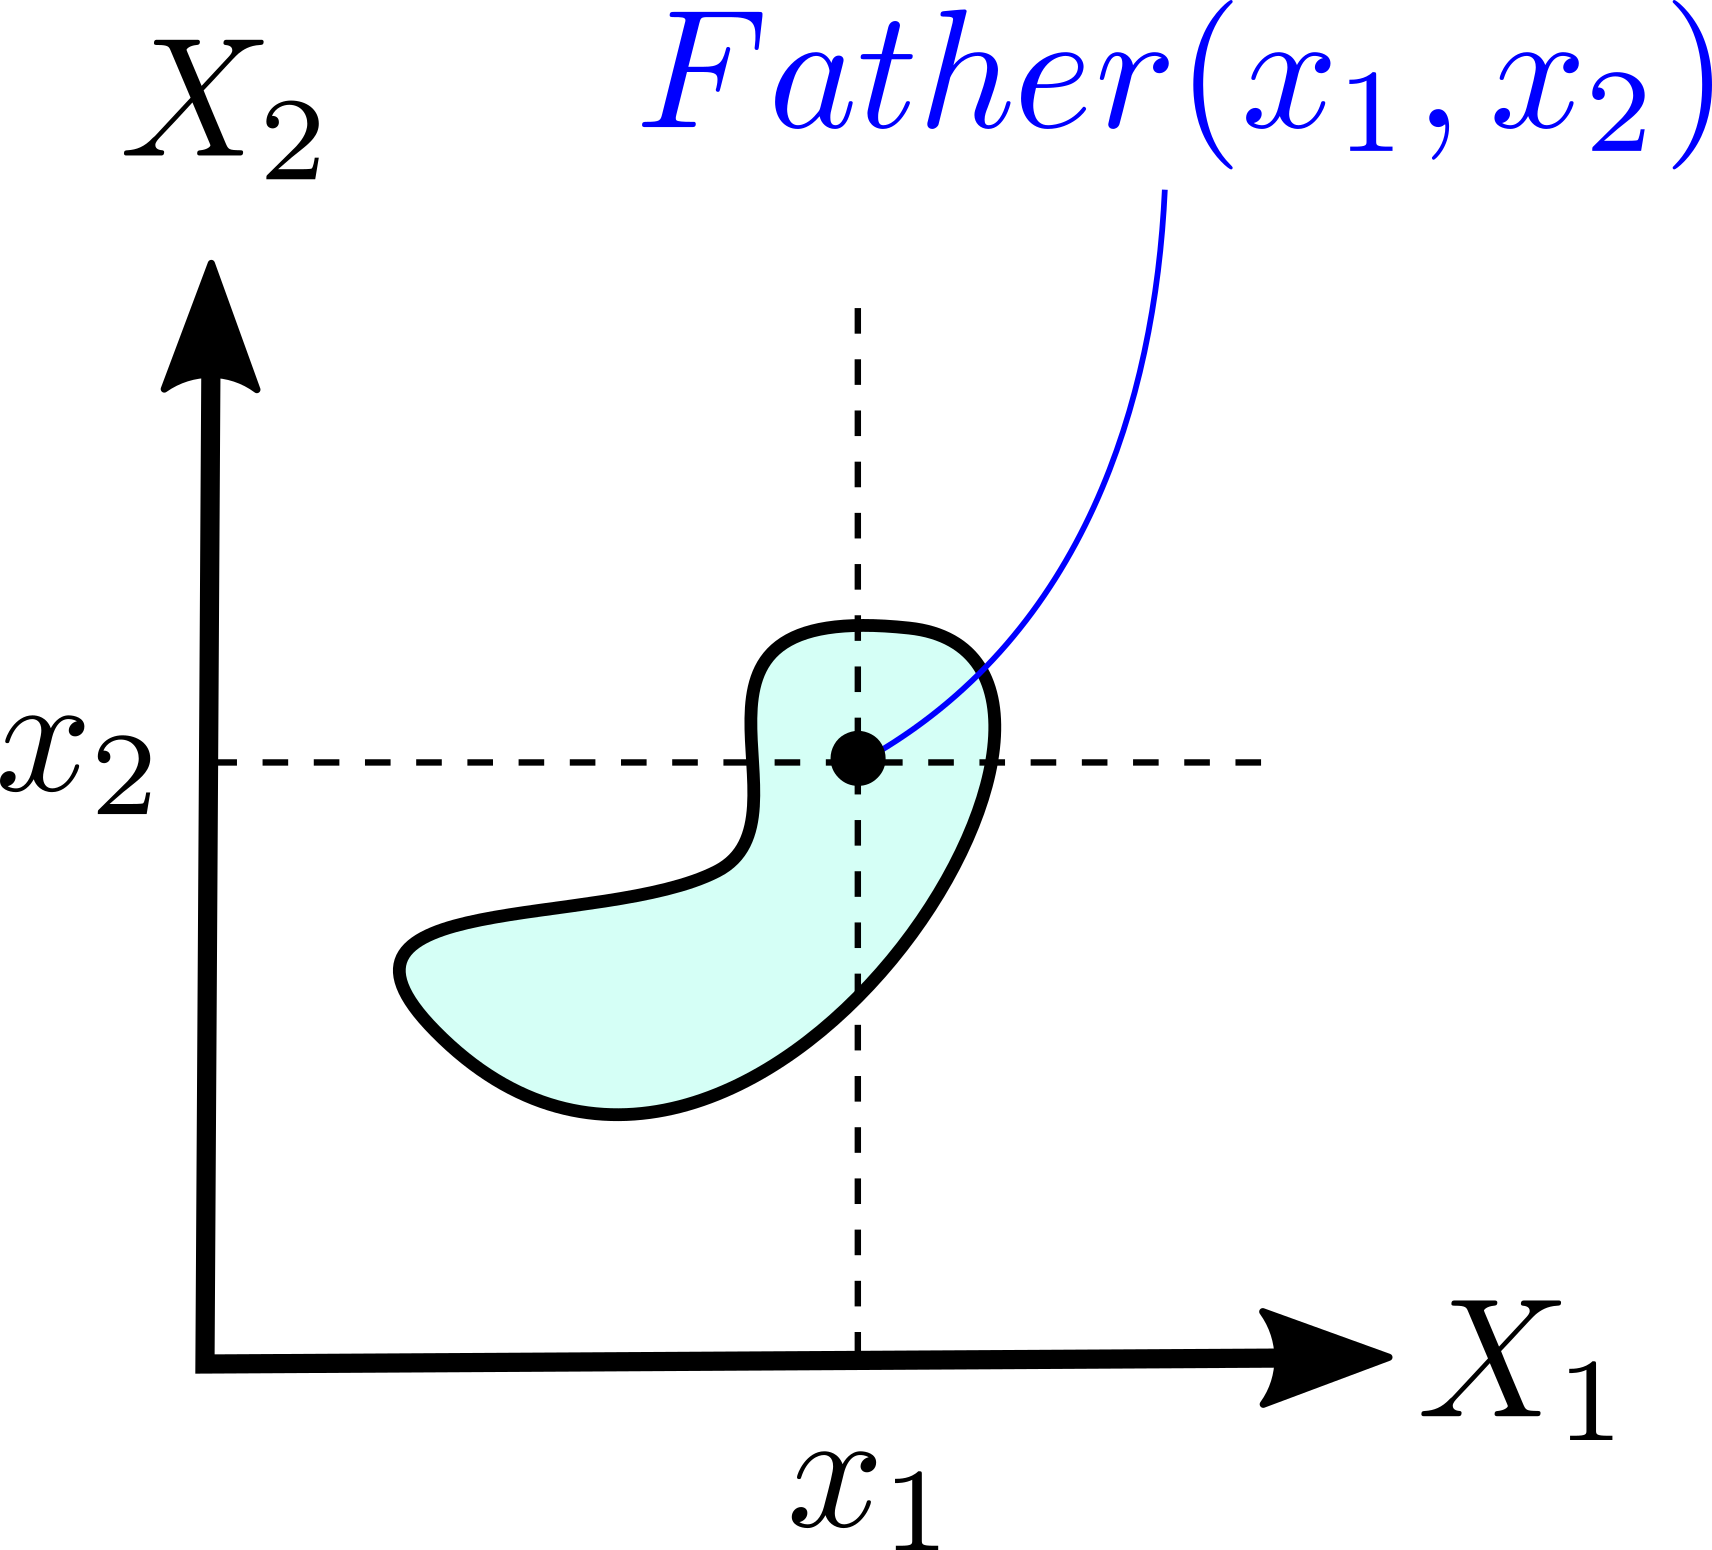
\includegraphics[scale=0.6]{cylindric-relation.png}}}
\quad \quad \quad
\vcenter{\hbox{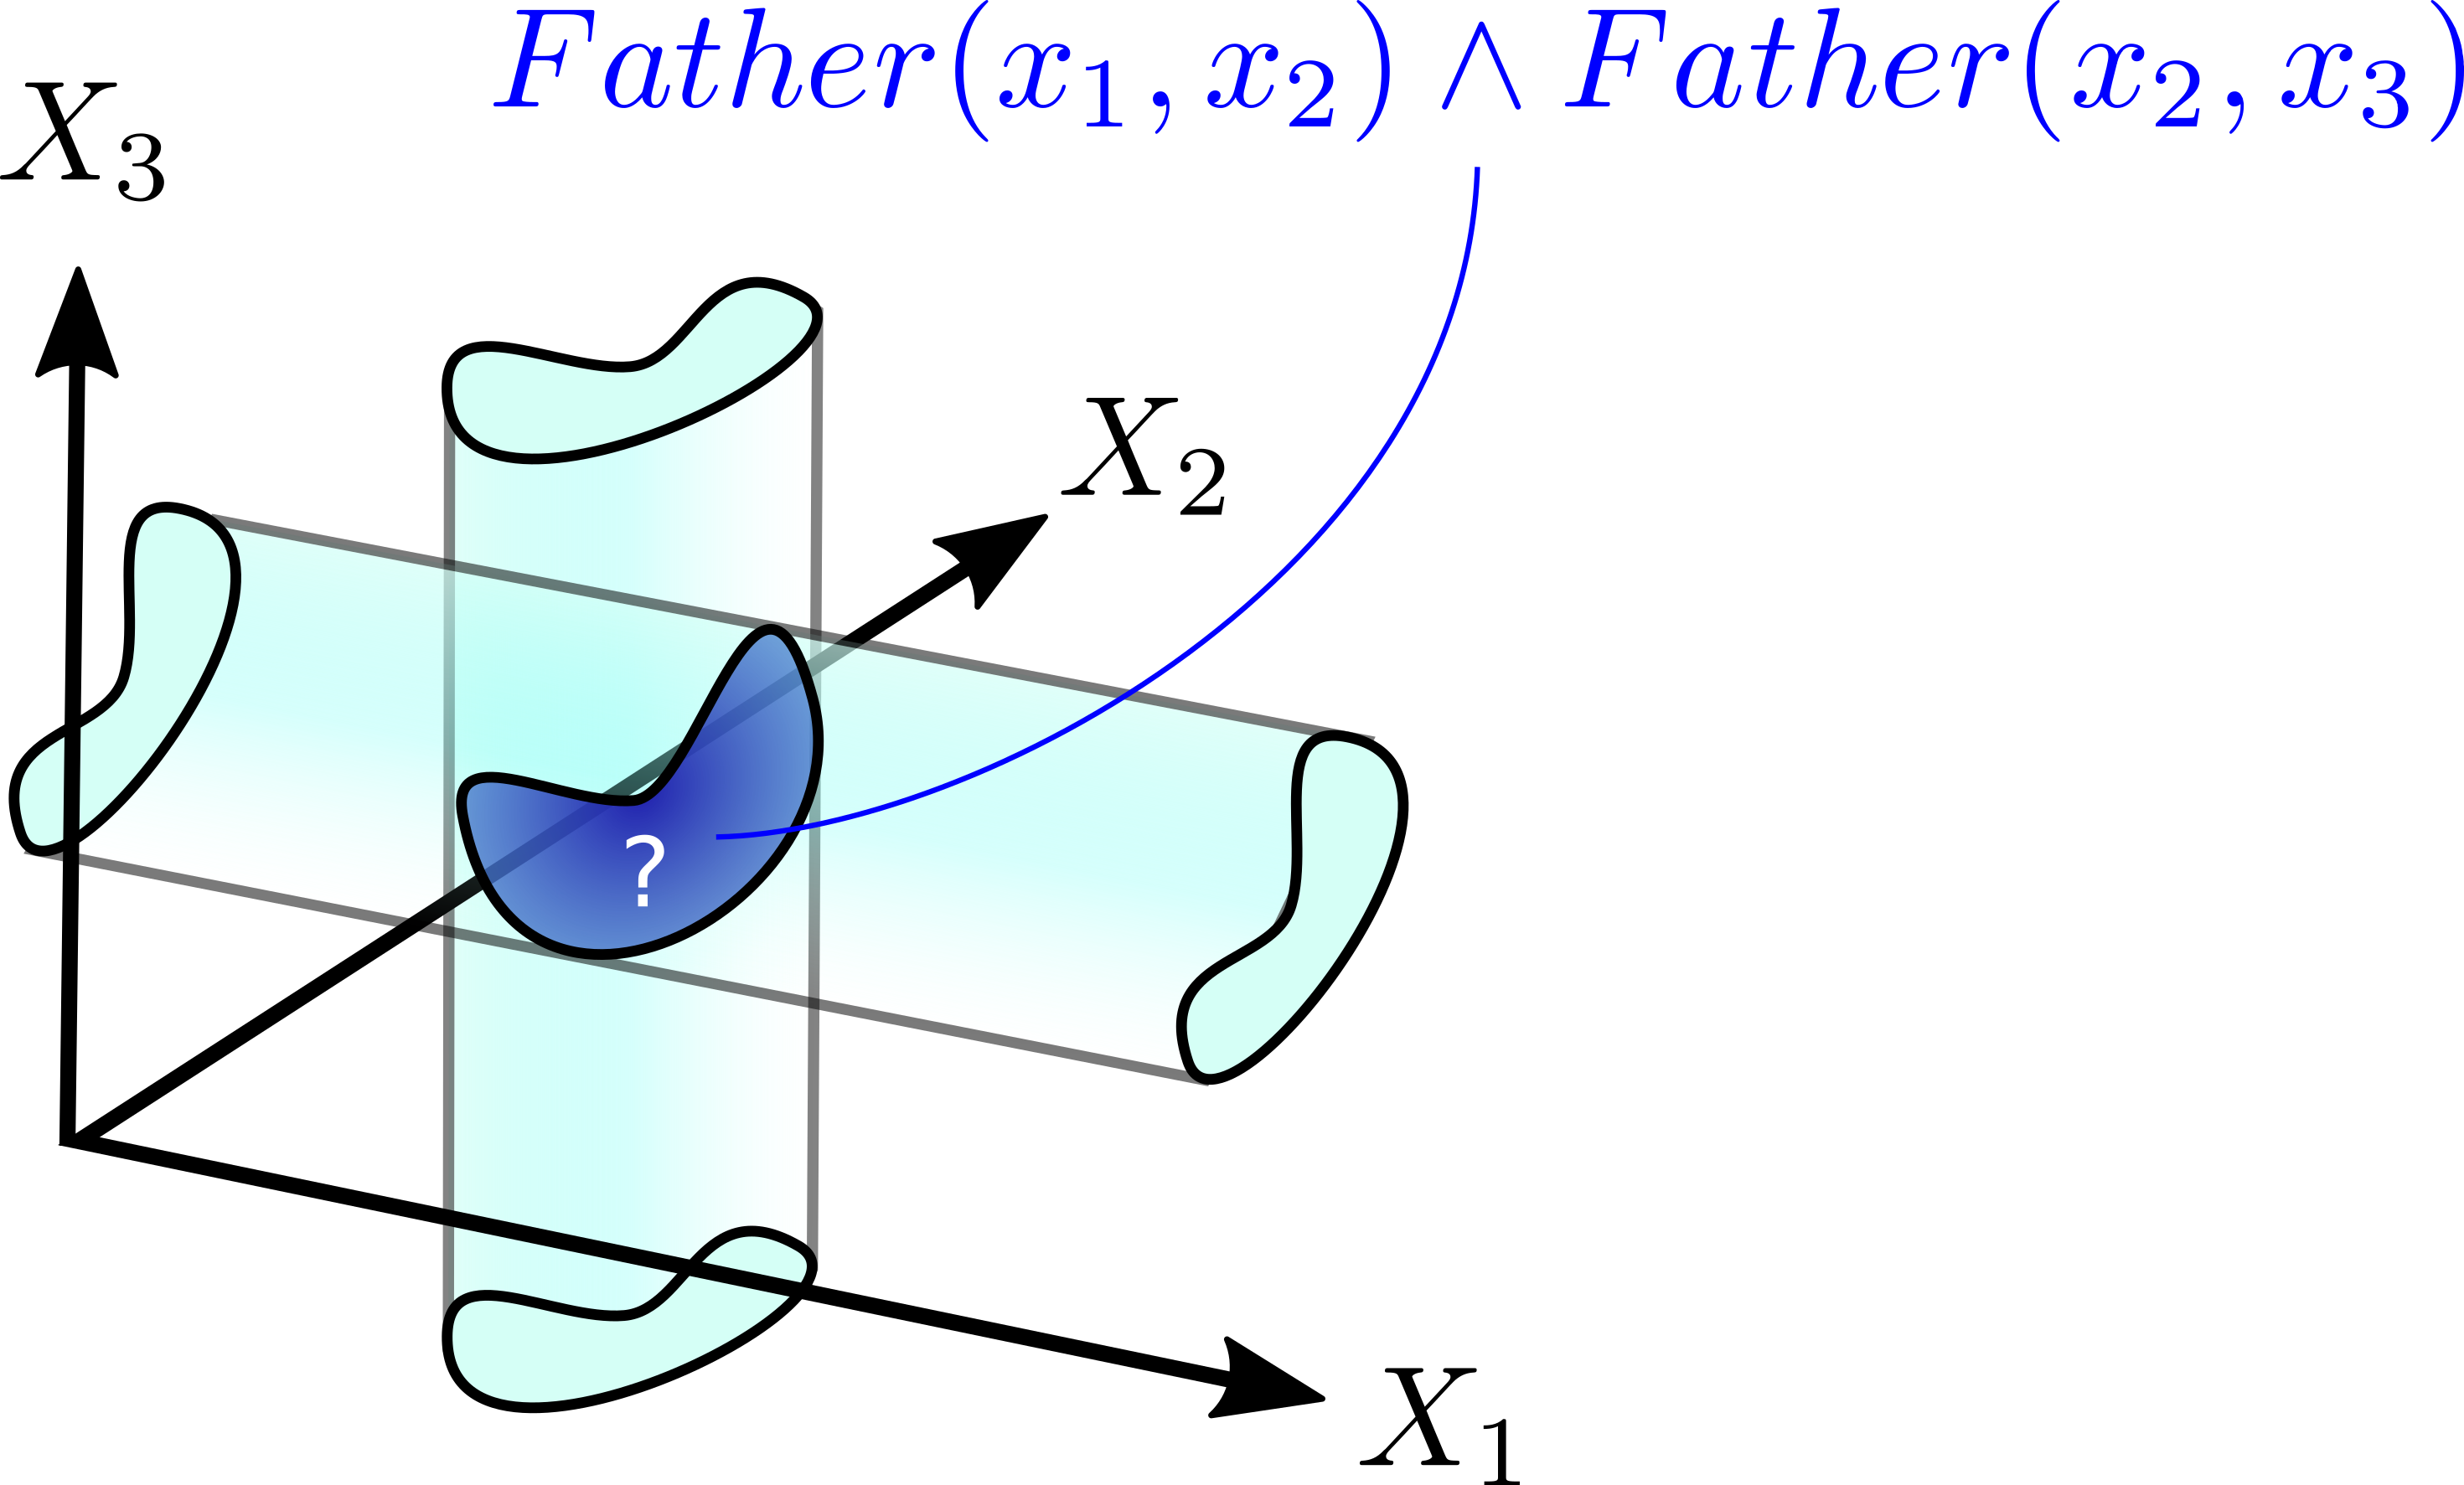
\includegraphics[scale=0.6]{cylindric-relation-intersection.png}}}
\end{equation}
And ``linkages'' cause the graph of the $\vdash$ map to \textit{pass through} diagonal lines such as follows:
\begin{equation}
\label{eqn:diagonal-shapes}
\vcenter{\hbox{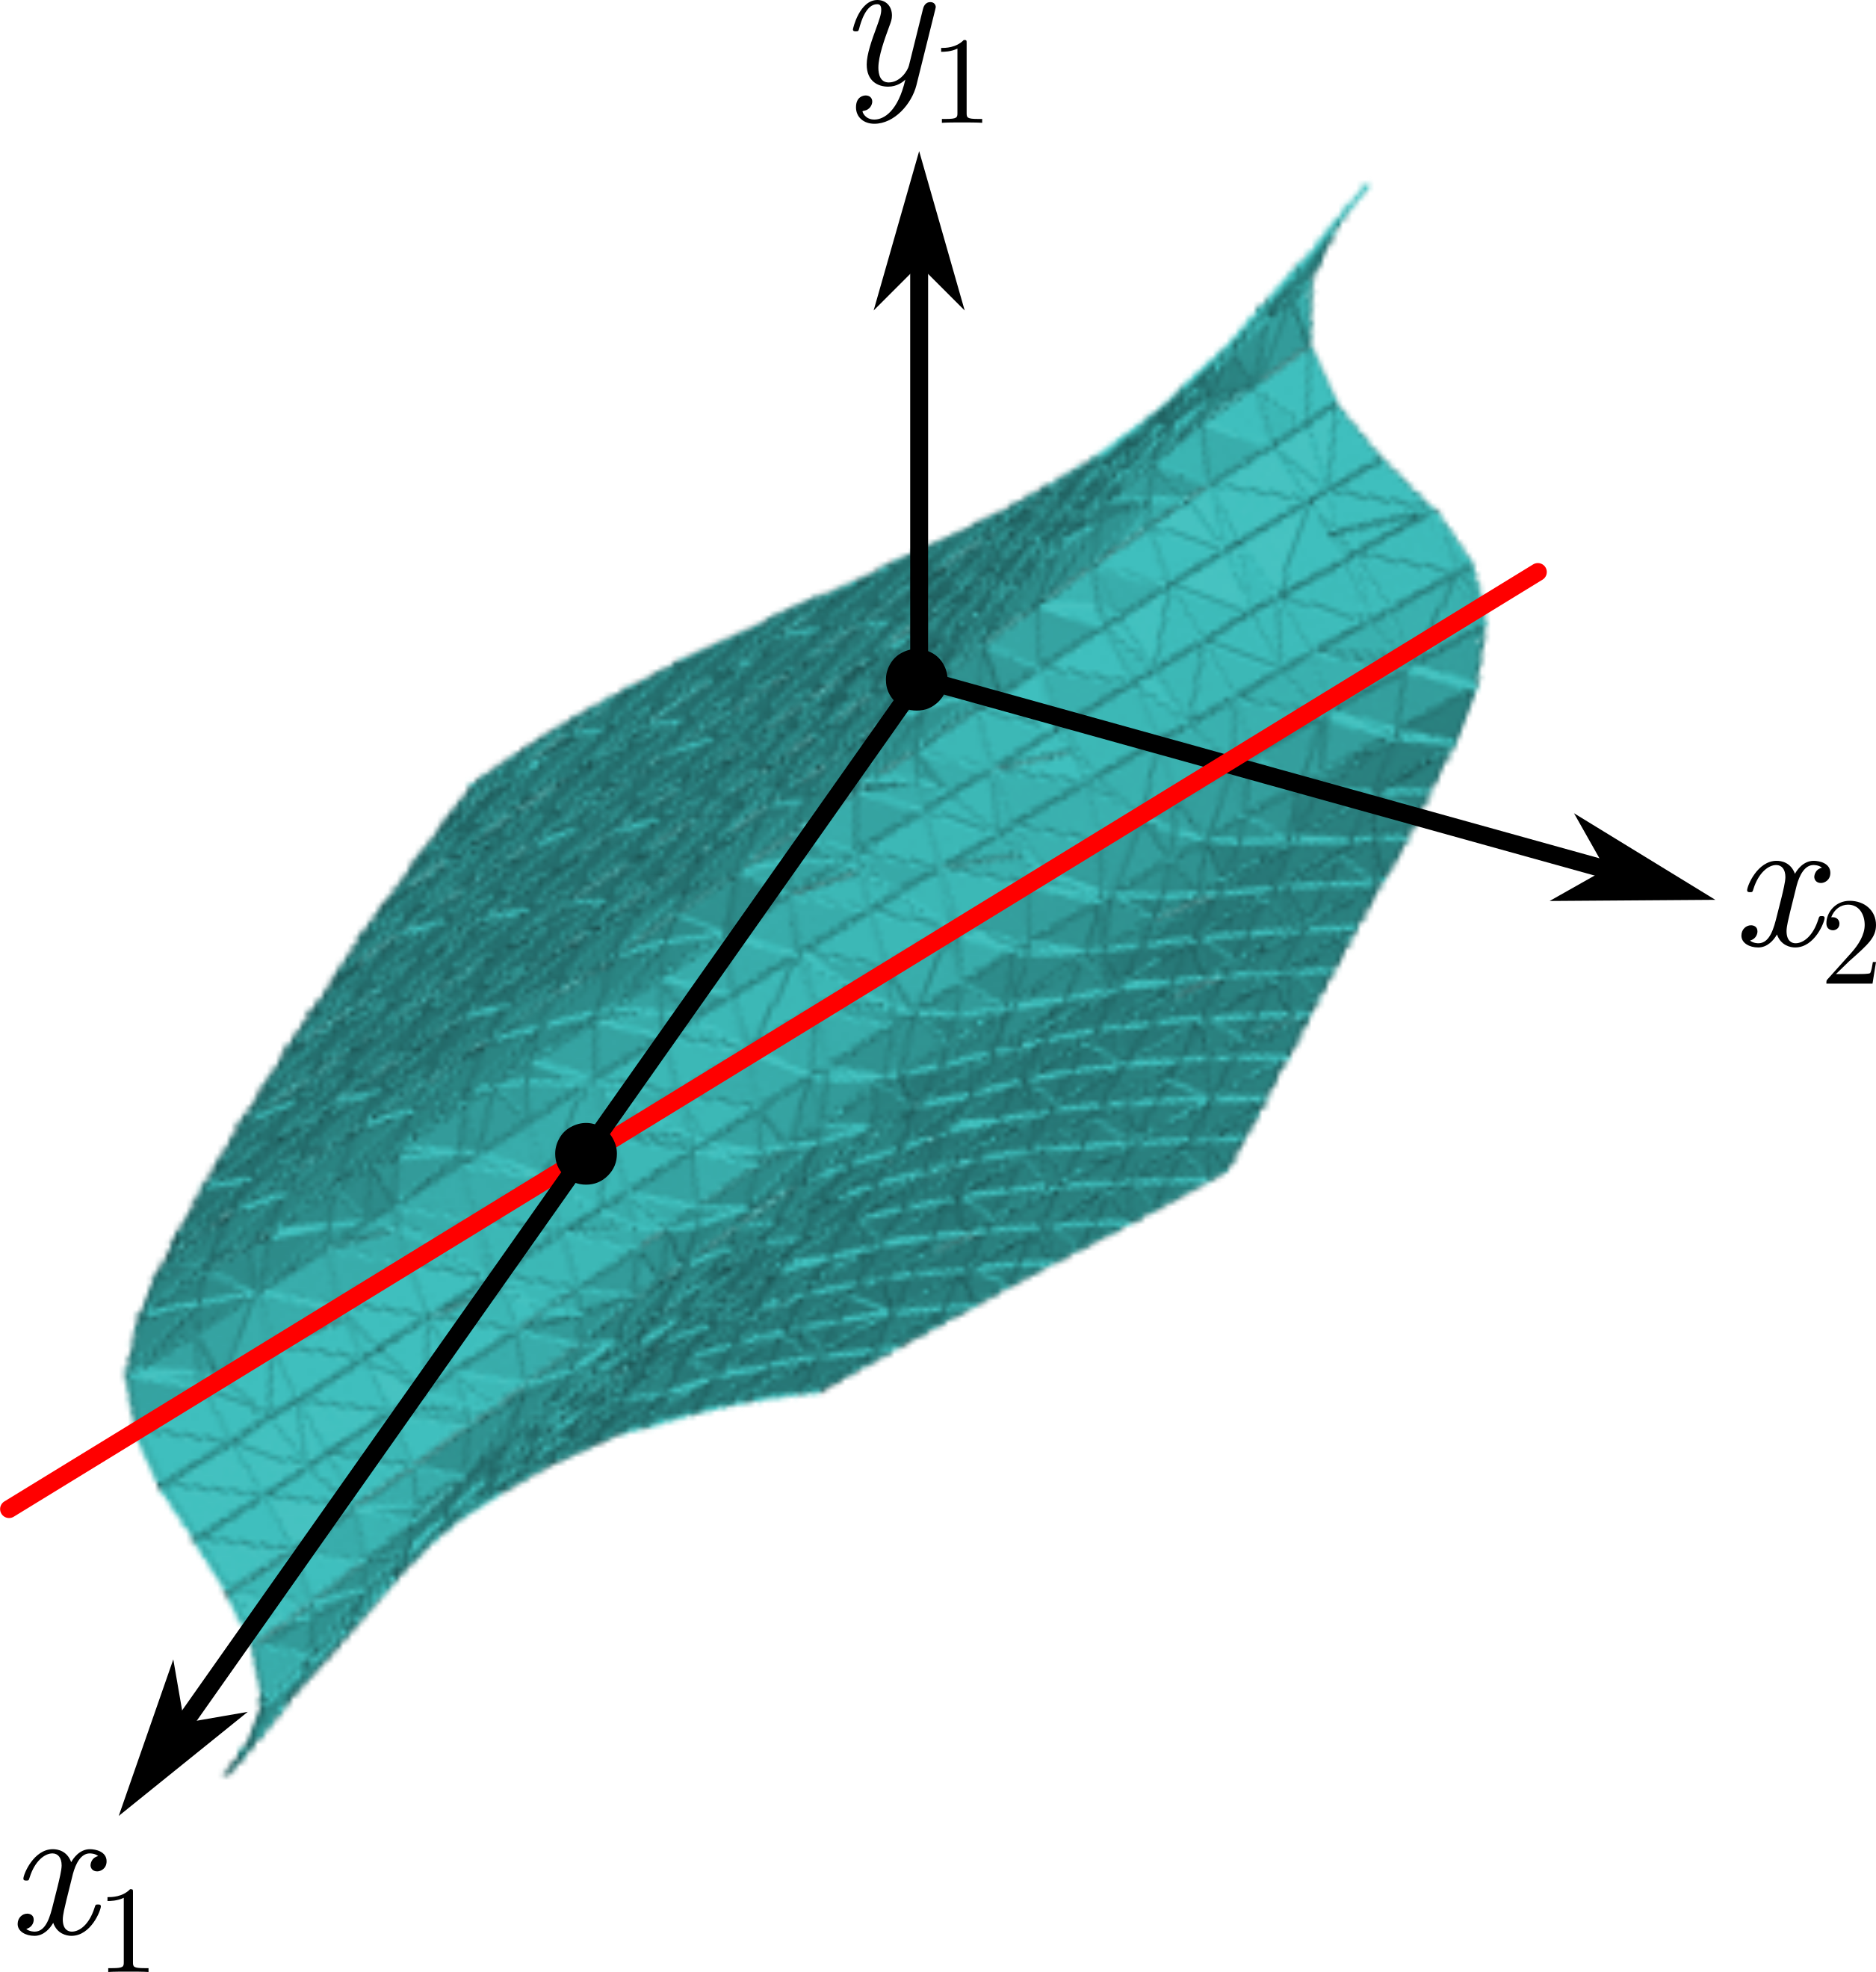
\includegraphics[scale=0.3]{diagonal.png}}}
\end{equation}
We are trying to use neural networks to approximate such functions (\textit{ie}, these geometric shapes).  One can visualize, as the shape of neural decision-boundaries approximate such diagonals, \uline{the matching of first-order objects gradually go from partial to fully-quantified} $\forall$ and $\exists$.  This may be even better than if we fix the logic to have exact quantifications, as quantified rules can be learned gradually.  %Since NNs are universal function approximators, they can in principle achieve that. 
There is also \textit{empirical} evidence that NNs can well-approximate logical maps, because the \textit{symbolic} matching and substitution of logic variables is very similar to what occurs in \textit{machine translation} between natural languages;  In recent years, deep learning is fairly successful at the latter task.

\subsection{Form of a logic rule}

So what exactly is the logic structure? Recall that inside our RL model:
\begin{itemize}
	\item state $\vect{x} \in \mathbb{X}$ = mental state = set of logic propositions $\vect{p} \in \mathbb{P}$
	\item environment = state space $\mathbb{X}$ = mental space
	\item actions $\vect{a} \in \mathbb{A}$ = logic rules
\end{itemize}

For our current prototype system, an action = a logic \textbf{rule} is of the form:
\newcommand{\Atom}{\,\mathsf{C}}
\renewcommand{\!}{\mkern6mu}
\begin{equation}
\label{eqn:logic-rule}
\overbrace{ \Atom^1_1 \Atom^1_2 \Atom^1_3 \! \wedge \! \underbrace{\Atom^2_1 \Atom^2_2 \Atom^2_3}_{\makebox[0pt]{each literal made of $m$ atomic concepts, $m = 3$ here}}  \! \wedge \! .... \! \wedge \! \Atom^k_1 \Atom^k_2 \Atom^k_3}^{\mbox{conjunction of $k$ literal propositions}} \quad \Rightarrow \quad \overbrace{ \Atom^0_1 \Atom^0_2 \Atom^0_3 }^{\mbox{conclusion}}
\end{equation}
where a \textbf{concept} can be roughly understood as a \textbf{word vector} as in Word2Vec.  Each $\Atom \in \mathbb{R}^d$ where $d$ is the dimension needed to represent a single word vector or concept.

We use a ``free'' neural network (\textit{ie}, standard feed-forward NN) to approximate the set of \textit{all} rules.  The \textbf{input} of the NN would be the state vector $\vect{x}$:
\begin{equation}
\Atom^1_1 \Atom^1_2 \Atom^1_3 \! \wedge \! \Atom^2_1 \Atom^2_2 \Atom^2_3 \! \wedge \! .... \! \wedge \! \Atom^k_1 \Atom^k_2 \Atom^k_3 .
\end{equation}
We fix the number of conjunctions to be $k$, with the assumption that conjunctions of length $< k$ could be filled with ``dummy'' (always-true) propositions.

The \textbf{output} of the NN would be the conditional \textbf{probability} of an action:
\begin{equation}
P(\mbox{action } | \mbox{ state}) := \pi(\Atom_1 \Atom_2 \Atom_3 \; | \; \vect{x}).
\end{equation}
Note that we don't just want the action itself, we need the \textbf{probability distribution} over these actions.  The \textbf{Bellman update} of reinforcement learning should update the probability distribution over such actions.

%\section{Implementation issues}

% Mathematically, a \textbf{neural network} is a non-linear function with many parameters (called ``weights'', organized as layers of matrices):
%\begin{eqnarray}
%\mbox{\footnotesize each layer's } \tikzmark{ww} \mbox{\footnotesize \textbf{weight} matrix} \quad \quad \mbox{\footnotesize total \# of layers} \tikzmark{LL} \nonumber \\
%\nonumber \\
%\vect{F}(\vect{x}) = \sigmoid(W_1 \tikzmark{wa} \sigmoid(W_2 \tikzmark{wb} ... \sigmoid( W_L \tikzmark{wc} \tikzmark{L} \; \vect{x} )))
%\begin{tikzpicture}[overlay,remember picture]
%\draw[-, shorten <=26pt, transform canvas={shift={(-10pt,10pt)}}] (ww.center) to (wa.center);
%\draw[-, shorten <=38pt, transform canvas={shift={(-10pt,10pt)}}] (ww.center) to (wb.center);
%\draw[-, shorten <=46pt, transform canvas={shift={(-10pt,10pt)}}] (ww.center) to (wc.center);
%\draw (LL.center) +(-15pt,-3pt) -- ([shift={(-2pt,6pt)}]L.center);
%\end{tikzpicture}
%\end{eqnarray}
%where $\sigmoid$ is a sigmoid-shaped non-linear function, applied component-wise to the vectors.

\subsection{Structure of a logic-based AI system}

Besides the intrinsic structure of a logic, the AI system has a structure in the sense that it must perform the following operations iteratively, in an endless loop:
\begin{equation}
\vcenter{\hbox{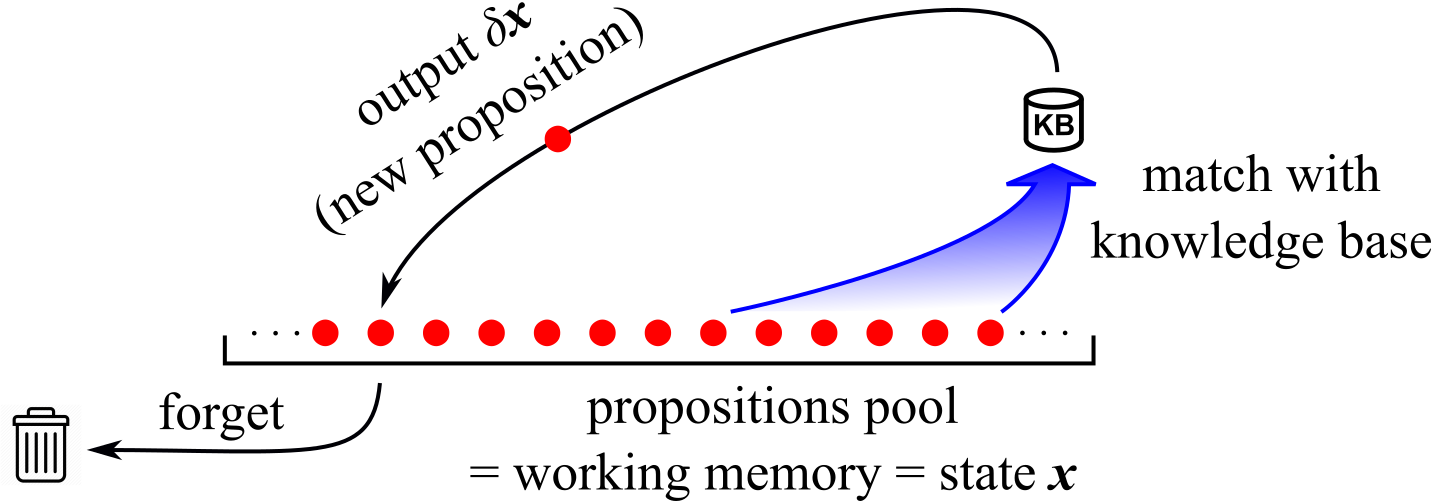
\includegraphics[scale=0.6]{classical-AI-architecture.png}}}
\end{equation}
\begin{itemize}
	\item \textbf{Matching} --- the $\KB$ of rules is matched against the current state $\vect{x}$, resulting in a (stochastically selected, \textit{eg} based on $\epsilon$-greedy) rule
		\begin{eqnarray}
		\boxed{\mbox{Match}} \quad
		( \vect{x} \stackrel{?}{=} \KB ) \;: \mathbb{X} &\rightarrow& ( \mathbb{X} \rightarrow \mathbb{P} ) \nonumber \\
		\label{eqn:matching}
		\vect{x} &\mapsto& \vect{r} 
		\end{eqnarray}
	--- In categorical logic, matching is seen as finding the \textbf{co-equalizer} of 2 terms which returns a \textbf{substitution}.  The substitution is implicit in our formulation and would be \textit{absorbed} into the neural network in our architecture.  \\
	--- Matching should be performed over the entire \textbf{working memory} = the state $\vect{x}$ which contains $k$ literals.  This is combinatorially time-consuming.  The celebrated \textbf{\textit{Rete}} algorithm turns the set of rules into a tree-like structure which is efficient for solving (\ref{eqn:matching}).
	\item \textbf{Rule application} --- the rule is applied to the current state $\vect{x}$ to produce a new literal proposition $\delta \vect{x}$
		\begin{eqnarray}
		\boxed{\mbox{Apply}} \quad
		\vect{r} : \mathbb{X} &\rightarrow& \mathbb{P} \nonumber \\
		\vect{x} &\mapsto& \vect{r}(\vect{x}) = \delta \vect{x}
		\end{eqnarray}
	\item \textbf{State update} --- the state $\vect{x}$ is \textit{destructively} updated where one literal $\vect{p}_j \in \vect{x}$ at the $j$-th position is \textbf{forgotten} (based on some measure of attention / interestingness) and over-written with $\delta \vect{x}$
		\begin{equation}
		\boxed{\mbox{Update}} \quad
		\vect{x} = (\vect{p}_1, \vect{p}_2, ..., \vect{p}_k ) \mapsto (\vect{p}_1, \vect{p}_2, ..., \delta \vect{x}, ..., \vect{p}_k )
		\end{equation}
\end{itemize}
All these operations are represented by functions parameterized by some variables $\Theta$ and they must be made \textit{differentiable} for gradient descent.

\subsection{Commutative structure of logic conjunctions}
\label{sec:symmetricNN}

The logic conjuction $\wedge$ is \textbf{commutative}:
\begin{equation}
\vect{p} \wedge \vect{q} \quad \Leftrightarrow \quad \vect{q} \wedge \vect{p} .
\end{equation}
If we want to use a neural network to model the deduction operator $\vdash: \mathbb{P}^k \rightarrow \mathbb{P}$, where $\mathbb{P}$ is the space of literal propositions, then this function should be \textbf{symmetric} in its input arguments.

A simple fact:  If $\vect{F}(\vect{p},\vect{q})$ is any function, then
\begin{equation}
\vect{F}(\vect{p},\vect{q}) + \vect{F}(\vect{q},\vect{p}) \quad \mbox{or} \quad \vect{F}(\vect{p},\vect{q})  \vect{F}(\vect{q},\vect{p})
\end{equation}
would be symmetric functions in $(\vect{p},\vect{q})$.  This can be easily extended to $\mathbb{P}^k$.  % We will use the additive method.

Thus if $\vect{F}$ is a ``free'' neural network, we can create a symmetric NN (via addition):
\begin{equation}
\vect{F}_{\mathrm{sym}}(\vect{x}) = \frac{1}{k!} \sum_{\sigma \in \mathfrak{S}_k} \vect{F}(\sigma \cdot \vect{x})
\end{equation}
where $\mathfrak{S}_k$ is the symmetric group of $k$ elements, and $\vect{x} = \vect{p}_1 \wedge \vect{p}_2 \wedge ... \vect{p}_k$.  Back-propagation can be easily adapted to such symmetric NNs.  However, if $K$ is the size of working memory, it would require to perform forward propagation $k! \;_K C_k = \;_K P_k$ times for each step, which is computationally inefficient (the same reason why \textit{Rete} was needed in classical AI).

So we would not use this idea, but it is illustrative of the problem.

\subsection{Spectral representation of states}

Now consider another simple idea.  Suppose we have 3 vectors $(\vect{v}_1, \vect{v}_2, \vect{v}_3)$ in a 1-dimensional vector space $V$, and we attach a \textbf{truth value} $\top = 1$ to each vector.  Then we try to approximate the \textbf{graph} of truth values $\top(\vect{v})$ as a ``wave'' using Fourier or wavelet transform:
\begin{equation}
\vcenter{\hbox{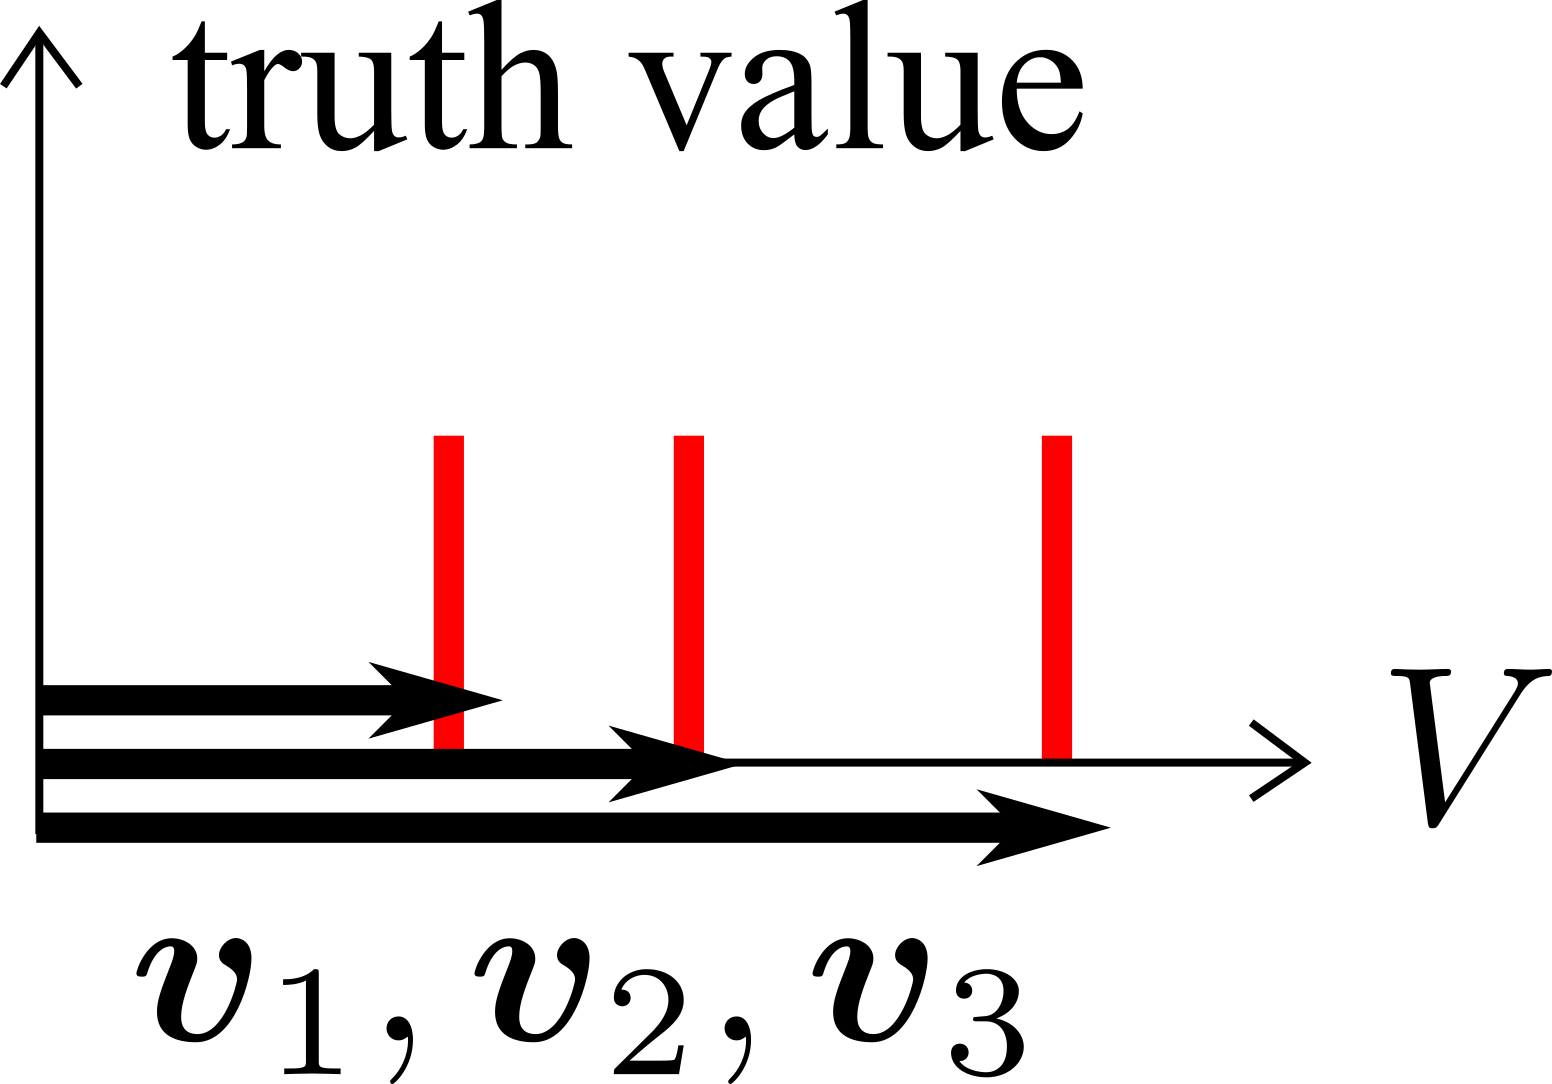
\includegraphics[scale=0.6]{Fourier-representation-0.png}}}
\quad \Rightarrow \quad
\vcenter{\hbox{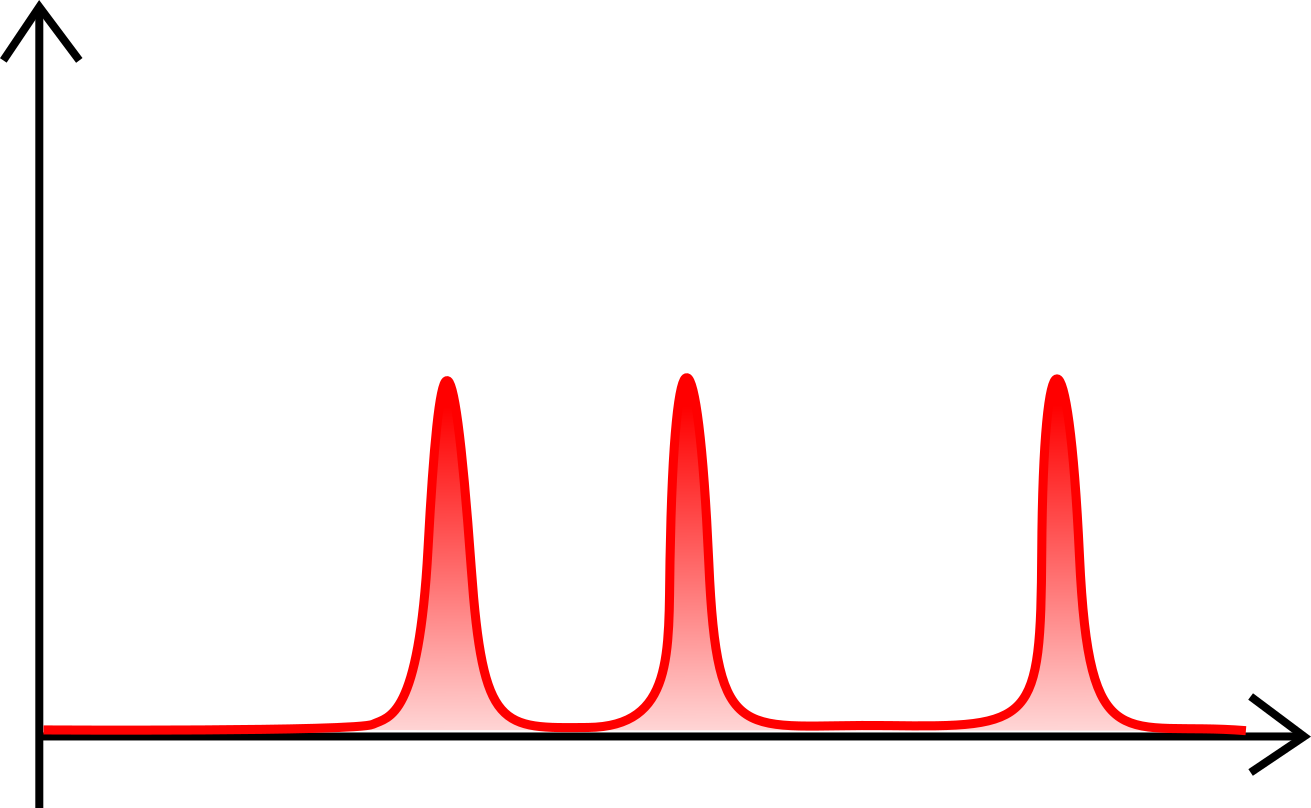
\includegraphics[scale=0.6]{Fourier-representation-0B.png}}}
\end{equation}

The resulting representation has some nice properties:
\begin{itemize}
	\item If we permute $(\vect{v}_1, \vect{v}_2, \vect{v}_3)$, the graph (and thus its spectrum) remains the same, \textit{ie}, the representation is \uline{invariant under permutations}
	\item We can add more vectors to the graph without changing the size of the spectral representation, \textit{ie}, it is relatively insensitive to the number of vectors
\end{itemize}

We can extend this idea to the \textbf{multi-dimensional} case where the literal proposition vector $\vect{p} \in \mathbb{P} = \mathbb{R}^{3d}$ 
\footnote{For example, a typical $d$ from Word2Vec or GloVe is 200, so $3d = 600$.}
and the state $\vect{x}$ consists of $k$ vectors $= \vect{p}_1 \wedge \vect{p}_2 \wedge ... \vect{p}_k$.  In other words, we need to apply Fourier transform to a wave over $3d$ dimensions.  Moreover, we can have truth values in the range $[-1,1]$, which can be construed as \textbf{fuzzy} truth values, or in the range $[0,1]$, regarded as the probability of \textbf{stochastic actions} (as is common in policy-gradient methods).
\begin{equation}
% \begin{tabular}{ccc}
% proposition vectors in $n$-dim space & & wave over $n$-dim space \\
% with {\color{red}truth values} \vspace*{0.5em} & & \\
\vcenter{\hbox{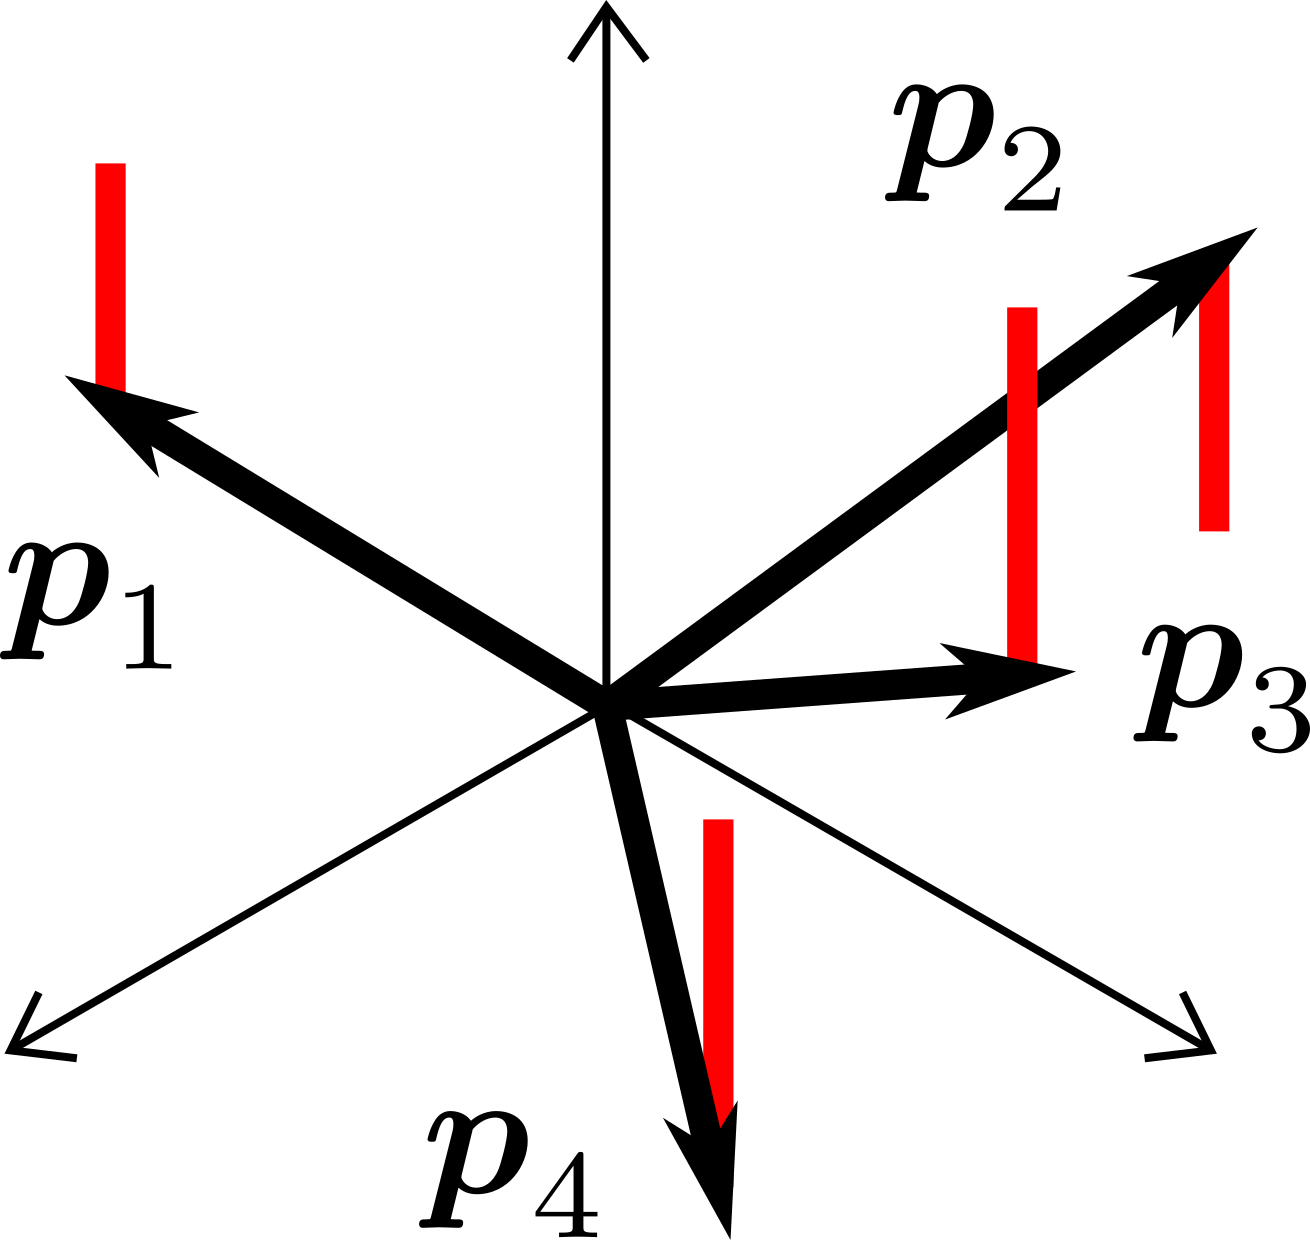
\includegraphics[scale=0.6]{Fourier-representation-1.png}}} 
\quad \Rightarrow \quad
\vcenter{\hbox{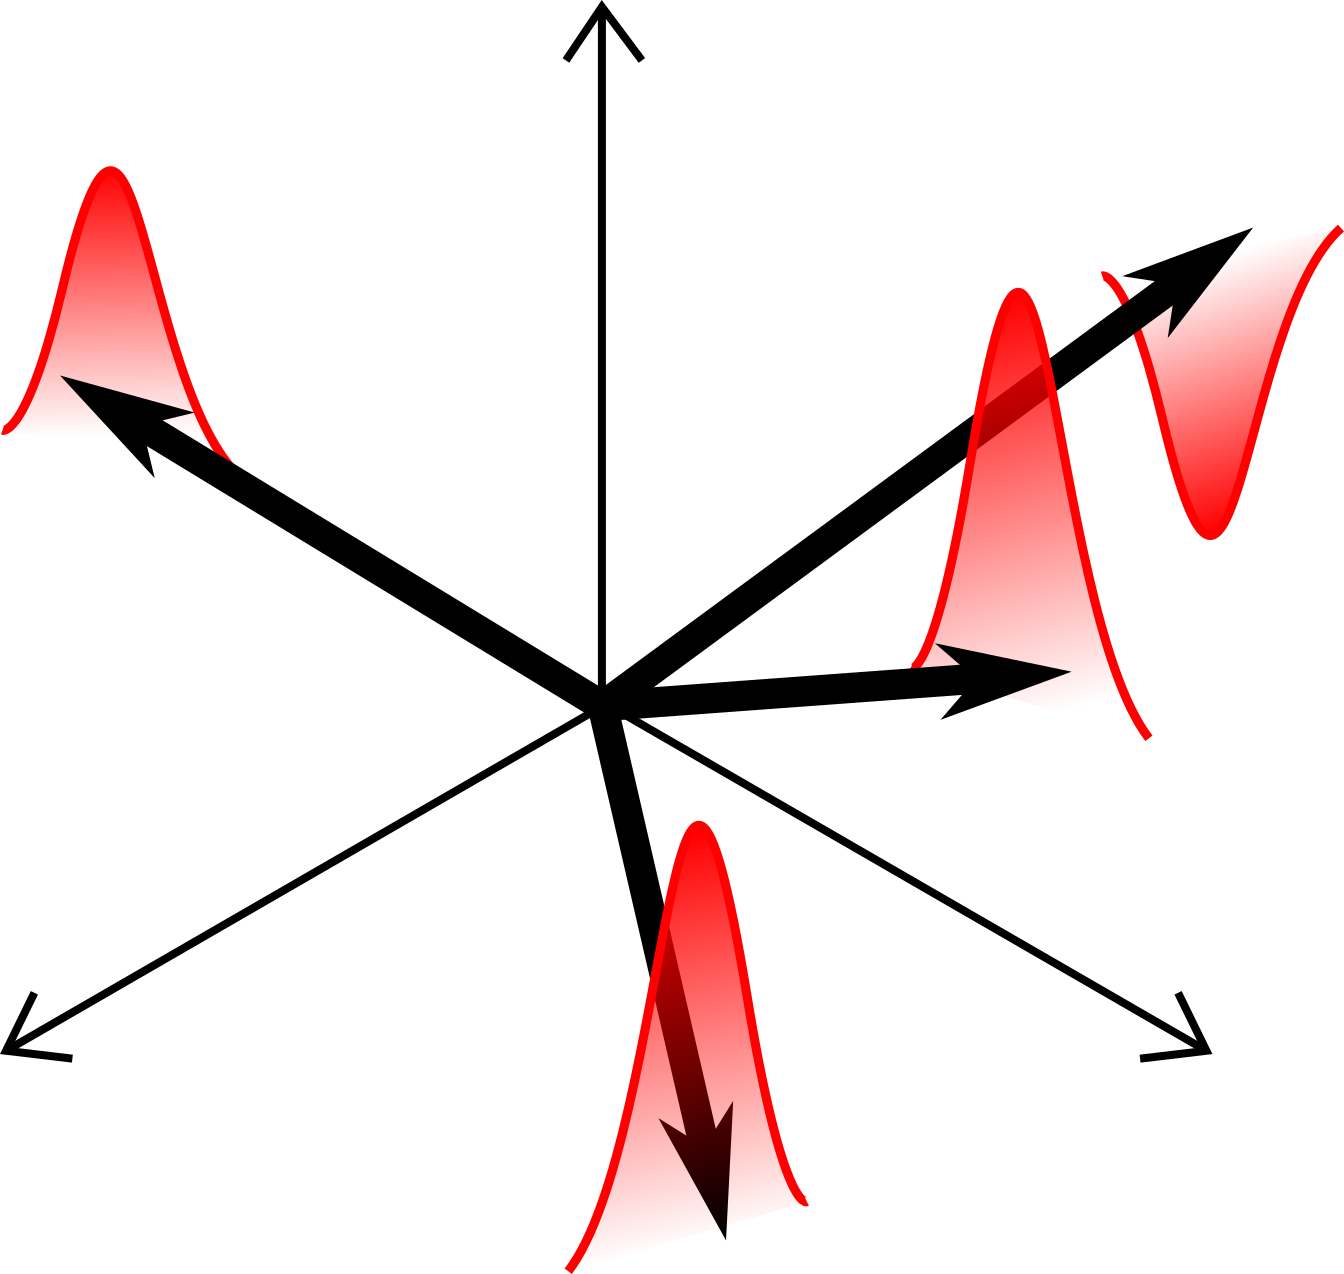
\includegraphics[scale=0.6]{Fourier-representation-2.png}}} 
% \end{tabular}
\end{equation}

Notice that our NN would \textit{input} from the spectral representation and \textit{output} the normal representation.

With this approach, the geometric shapes of (\ref{eqn:cylindric-shapes}) and (\ref{eqn:diagonal-shapes}) would be distorted in very complicated ways.  It remains to be verified whether NNs can learn this task effectively.

\subsection{Probability distribution over continuous actions}

All the ``knowledge'' of the agent is contained in the \textbf{policy} function $\pi$:
\begin{eqnarray}
\pi: \mathbb{X} \times \mathbb{A} &\rightarrow& [0,1] \in \mathbb{R} \nonumber \\
(\vect{x},\vect{a}) &\mapsto& P(\vect{a} \;|\; \vect{x})
\end{eqnarray}
where $\mathbb{X}$ = state space, $\mathbb{A}$ = action space, $P(\cdot)$ = conditional probability.

In reinforcement learning in general, the function space of $\pi$ is of shape:
\begin{equation}
\pi : \mathbb{X} \rightarrow \mathbb{R} (\mathbb{A}) = \mathbb{R}^{\mathbb{A}} .
\end{equation}
For example, if $\mathbb{A}$ has finitely 10 discrete actions, $\mathbb{R}(\mathbb{A})$ would be $\mathbb{R}^{10}$.  For logic-based agents, $\mathbb{A}$ would be the set of all logic rules, thus very large.  It would be worse if $\mathbb{A}$ is continuously-valued, as when we embed logic rules in vector space.

So we may use \textbf{Gaussian kernels} (\textit{ie}, radial basis functions) to approximate $\pi(\vect{a} | \vect{x})$:
\begin{equation}
P(\vect{a} | \vect{x}) \approx \hat{P}(\vect{a} | \vect{x}) := \frac{1}{N h} \sum_{i = 1}^{N} \Phi \left( \frac{\vect{a} - \vect{a}_i}{h} \right)
\end{equation}
where $\Phi(u)$ is the Gaussian kernel $\frac{1}{\sqrt{2 \pi}} e^{- u^2 / 2}$. 

For each state $\vect{x}$, our NN outputs a probabilistic \textit{choice} of $c$ actions.  So we only need to maintain $c$ ``peaks'' given by Gaussian kernels.  Each peak is determined by its mean $\vect{a}_i$ and variance (a scalar constant fixed globally as $h$).

TO-DO: The Gaussian kernels should be \textbf{weighted}.

An action $\vect{a} \in \mathbb{A}$ is a logic rule that takes the state $\vect{x}$ to a proposition $\vect{p}$, \textit{ie}, $\mathbb{A} = \mathbb{X} \rightarrow \mathbb{P}$.  When a rule is applied to a state, it becomes a proposition, so the space of \textit{applied} actions $\mathbb{A}(\vect{x})$ in our case is equivalent to $\mathbb{P}$.

Also, after our ``Fourier trick'', $\mathbb{X} = \mathbb{R}^{3dk}$ becomes $\widehat{\mathbb{X}} = \mathbb{R}^{3d}$ as the number of conjunctions $k$ is absorbed into $\widehat{\mathbb{X}}$.

% So our NN would be the function $\pi()(\vect{x})$ (with rules applied to $\vect{x}$):
% \begin{equation}
% \pi()(\vect{x}): \widehat{\mathbb{X}} \rightarrow (\mathbb{X}^c \times (\mathbb{X} \rightarrow (\mathbb{P} \rightarrow \mathbb{R}))^c)
% = \widehat{\mathbb{X}} \rightarrow (\mathbb{P} \rightarrow \mathbb{R})^c
% \end{equation}
% where
Each applied action $\vect{a}(\vect{x}) \in \mathbb{P}$ is of the form $\Atom_1 \Atom_2 \Atom_3$ and is of size $\mathbb{R}^{3d}$, as explained in (\ref{eqn:logic-rule}).  Thus our NN has the shape:
\begin{eqnarray}
\pi()(\vect{x}): \widehat{\mathbb{X}} \rightarrow (\mathbb{P} \rightarrow \mathbb{R})^c
% \quad = \quad (\mathbb{R}^{3d})^k \rightarrow (\mathbb{R}^{3d})^c
\quad = \quad \mathbb{R}^{3d} \rightarrow (\mathbb{R}^{3d} \rightarrow \mathbb{R})^c .
\end{eqnarray}

% \subsection{Algorithm}

% The algorithm is exactly the same as the standard $Q$-learning algorithm:

%\begin{tcolorbox}[colback=grey, breakable, enhanced]
%\begin{lstlisting}
%Initialize all $Q(x,a)$ arbitrarily
%For all episodes
%    Initialize $x$
%    Repeat
%        Choose $a$ using policy derived from $Q$, eg $\epsilon$-greedy
%        Take action $a$, observe $R$ and $x'$
%        Update $Q(x,a)$:
%            $ Q(x,a) \stackrel{+}{=} \eta \left[ R + \gamma \displaystyle\max_{a'} Q(x',a') - Q(x,a) \right] $
%        $ x \leftarrow x' $
%    Until $x$ is terminal state
%\end{lstlisting}
%\end{tcolorbox}

\section{Conclusion and future directions}

This paper has 2 main contributions:
\begin{itemize}
	\item The use of Hamiltonian maximization gradient descent for deep reinforcement learning
	\item Spectral representation of logic states $\vect{x}$ to achieve commutativity
\end{itemize}

\bibliographystyle{plain} % or number or aaai ...
\bibliography{../AGI-book}

\end{document}
